% -*-LaTex-*-

%-----------------------------------------------------------------------------
%   Copyright 2015 Florian Schumacher
%
%   This file is part of the ASKI manual as a LaTeX document with main file
%   manual.tex
%
%   Permission is granted to copy, distribute and/or modify this document
%   under the terms of the GNU Free Documentation License, Version 1.3
%   or any later version published by the Free Software Foundation;
%   with no Invariant Sections, no Front-Cover Texts, and no Back-Cover Texts.
%   A copy of the license is included in the section entitled ``GNU
%   Free Documentation License''. 
%-----------------------------------------------------------------------------
%
%#########################################################################
% ATTENTION: THERE ARE STILL SEVERAL PROBLEMS TO COMPILE THIS DOCUMENT RESULTING
% IN A LOT OF WARNINGS. YOU PROBABLY NEED TO COMPILE THIS DOCUMENT IN MODE 
% ``nonstopmode'' by:
% 
% pdflatex \\nonstopmode\\input manual.tex
% bibtex manual
% pdflatex \\nonstopmode\\input manual.tex
% pdflatex \\nonstopmode\\input manual.tex
% pdflatex \\nonstopmode\\input manual.tex
% 
%#########################################################################



%#########################################################################
%%   TODO DOCUMENTATION:
%% 
%%  ->  put text boxes for ``simple solution'' and ``advanced options'', where applicable
%% 
%%  ->  possible name for successor program package:
%%         ANSI - ANalysis of Sensitivity and Inversion
%%      with regard to the common (however, not official) name ``ANSI'' of a group of 
%%      ASCII-based 8-byte character sets like Latin 1, UTF-8.
%% 
%#########################################################################


\documentclass[12pt,a4paper]{book}

\usepackage[english]{babel} %language selection
\selectlanguage{english}

\pagenumbering{arabic}

\usepackage[affil-it]{authblk}
\usepackage{times} % 'times new roman' script style

\usepackage{amsmath}
\usepackage{amssymb}
\usepackage[pdftex]{graphicx}

% use package url with [obeyspaces] in order to correctly display \nolinkurl WITH spaces 
%(used in \newcommand{\lcode} below). As hyperref internally loads package url, you can pass
% option obeyspaces of package url to package hyperref as follows
\PassOptionsToPackage{obeyspaces}{url}\usepackage{hyperref}
%\hypersetup{colorlinks, 
%           citecolor=black,
%           filecolor=black,
%           linkcolor=black,
%           urlcolor=black,
%           bookmarksopen=true,
%           pdftex}
%\hfuzz = .6pt % avoid black boxes

% the following is an ugly solution of allowing line breaks in urls additionally after every normal 
% alphabetic character which (if \nolinkurl is used in \newcommand{\lcode} below) at all allows line 
% breaks of long routine names like 'transformToStandardCellInversionGrid', BUT of course also breaks
% any other term formatted by \lcode at any character, which is maybe not very nice.
%\let\origUrlBreaks\UrlBreaks
%\renewcommand*{\UrlBreaks}{\origUrlBreaks\do\a\do\b\do\c\do\d\do\e\do\f\do\g\do\h\do\i\do\j\do\k\do\l\do\m\do\n\do\o\do\p\do\q\do\r\do\s\do\t\do\u\do\v\do\w\do\x\do\y\do\z\do\A\do\B\do\C\do\D\do\E\do\F\do\G\do\H\do\I\do\J\do\K\do\L\do\M\do\N\do\O\do\P\do\Q\do\R\do\S\do\T\do\U\do\V\do\W\do\X\do\Y\do\Z}


%% POSSIBLE PACKAGES TO DISPLAY CODE
%%
%% package alltt: verbatim environment within which math is displayed correctly
%% usage: \begin{alltt}\end{alltt}
%\usepackage{alltt}
%%
%% package listings: provides environments to display code fragments (with a lot of special characters) in a more evolved fashion than verbatim (alltt)
%% only uncomment (both next lines), if used in \newcommand{\lcode} below
\usepackage{listings}
\lstset{basicstyle =\ttfamily}%\small}

\usepackage[paperwidth=21.0cm,paperheight=29.7cm, left=2.5cm,right=2.5cm,top=2.0cm,
            bottom=2.0cm,headheight=0in,footskip=1.0cm]{geometry}
%-------------------------------
%
% COMMANDS FOR IN-LINE PHRASES IN CODE-STYLE
%
%%% ttfamily does not properly support any special characters
%\newcommand{\lcode}[1]{ {\ttfamily #1 }}
%
%%% lstinline is a good solution, in general, but it makes problems in line breaks!
%\newcommand{\lcode}[1]{\lstinline[breaklines=true]$#1$}
%
%%% although there are no actual links, it uses the same font as lstinline (when \lstset{basicstyle =\ttfamily}), 
%%% but produces better line breaks!
\newcommand{\lcode}[1]{\nolinkurl{#1}}
%
%%% need \lcodetitle, since \nolinkurl in a title of a numerated (sub)section (not *) causes problems in bookmark 
%%% view in adobe reader (why?! what is the actual problem?), \lcodetitle, however, does NOT support stuff like '_' etc.
\newcommand{\lcodetitle}[1]{ {\ttfamily #1} }
%
%
\newcommand{\ASKI}{ {\ttfamily ASKI} }
%
%
% OTHER NEW COMMANDS
%
\newcommand{\inotice}[1]{ \fbox{\parbox[t]{0.9\textwidth}{{\bf Important:} \\#1}} }
\newcommand{\notice}[1]{ \fbox{\parbox[t]{0.9\textwidth}{#1}} }
\newcommand{\myref}[1]{\ref{#1} (page~\pageref{#1})}
\newcommand{\myaref}[1]{$\rightarrow$~\ref{#1} (page~\pageref{#1})}
%
\newcommand{\vecthree}[3]{
  \begin{pmatrix}
    #1 \\ #2 \\ #3
  \end{pmatrix}
}
\newcommand{\weights}{$w_1,\dots,w_{n_c}$}
\newcommand{\weightsS}{$w^S_1,\dots,w^S_{n_c}$}
\newcommand{\wpG}{$\mathbf{x}_1,\dots,\mathbf{x}_{n_c}$}
\newcommand{\wpS}{$\mathbf{x}^S_1,\dots,\mathbf{x}^S_{n_c}$}
\newcommand{\RRR}{\mathbb{R}^3}
\newcommand{\Rd}{\mathbb{R}^d}
\newcommand{\R}[1]{$\mathbb{R}^{#1}$}
\newcommand{\brackr}[1]{\left( #1 \right)}
\newcommand{\brackg}[1]{\left\{ #1 \right\}}
%
%-------------------------------
%
% END OF PREAMBLE
%####################################################################
%
\begin{document}
%
\setlength{\parindent}{0em}
\setlength{\parskip}{0.5em}
% TeX's first attempt at breaking lines is performed without even trying hyphenation: 
% TeX sets its "tolerance" of line breaking oddities to the internal value \pretolerance
% an "infinite" tolerance is represented by the value 10000, but may lead to very bad line breaks indeed!
%\pretolerance=10000
%
%-------------------------------
% TITLE PAGE(s)
%
%-----------------------------------------------------------------------------
%   Copyright 2013 Florian Schumacher
%
%   This file is part of the ASKI manual as a LaTeX document with main file
%   manual.tex
%
%   Permission is granted to copy, distribute and/or modify this document
%   under the terms of the GNU Free Documentation License, Version 1.3
%   or any later version published by the Free Software Foundation;
%   with no Invariant Sections, no Front-Cover Texts, and no Back-Cover Texts.
%   A copy of the license is included in the section entitled ``GNU
%   Free Documentation License''. 
%-----------------------------------------------------------------------------
%


%#########
% classical titlepage using \maketitle

%\title{\thispagestyle{empty} \tt {\Huge ASKI} {\rm --} {\Huge A}{\large nalysis of} {\Huge S}{\large ensitivity \\ and } {\Huge\tt K}{\large ernel} {\Huge\tt I}{\large nversion} \\ \vspace*{1cm} Version 0.3 \\ User Manual}
%\title{\thispagestyle{empty} \tt {\Huge ASKI} {\rm --} version 0.3 \\ User Manual}

% without \usepackage[affil-it]{authblk} e.g.:
%\author{Florian Schumacher \thanks{\texttt{florian.schumacher@rub.de}; corresponding author} \and Wolfgang Friederich \thanks{\texttt{wolfgang.friederich@rub.de}}}
% WITH authblk:
%\author[1]{Florian Schumacher, Wolfgang Friederich}
%\author[1]{Florian Schumacher \thanks{\texttt{florian.schumacher@rub.de}; corresponding author}}
%\author[1]{Wolfgang Friederich \thanks{\texttt{wolfgang.friederich@rub.de}}}
%\affil[1]{Ruhr-Universit\"at Bochum} % for this you need \usepackage[affil-it]{authblk}

%\date{\today}
%\date{6.12.2004}
%\date{} % no date

%\maketitle
% END classical titlepage using \maketitle
%#########




%#########
% individual titlepage using \begin{titlepage},\end{titlepage}
\begin{titlepage}
\thispagestyle{empty}

  \begin{center}
    \tt \Huge ASKI
  \end{center}
  \vspace*{2cm}

  \begin{minipage}{0.5\textwidth}
    \begin{flushleft}
      \fontsize{20}{40} \selectfont
      {\tt {\Huge A}{\large nalysis of} \\ {\Huge S}{\large ensitivity and } \\ {\Huge\tt K}{\large ernel} \\ {\Huge\tt I}{\large nversion} }
    \end{flushleft}
  \end{minipage}
  \hfill
  \begin{minipage}{0.5\textwidth}
    \begin{flushright}
      {\fontsize{20}{40} \selectfont \tt {\Huge User Manual} \\  ASKI {\rm --} {\large version 1.0} \\ {\large Dec 2015} \\}
      %{\tt {\large Florian Schumacher \\Wolfgang Friederich} \\ {\small Ruhr-Universit\"at Bochum, Germany} }
      {\tt {\large Florian Schumacher \\ {\small Ruhr-Universit\"at Bochum, Germany} }
    \end{flushright}
  \end{minipage}

\vspace*{3cm}
%\vfill

\begin{center}
  \setlength{\fboxsep}{0pt}%
  \setlength{\fboxrule}{2pt}%
  \fbox{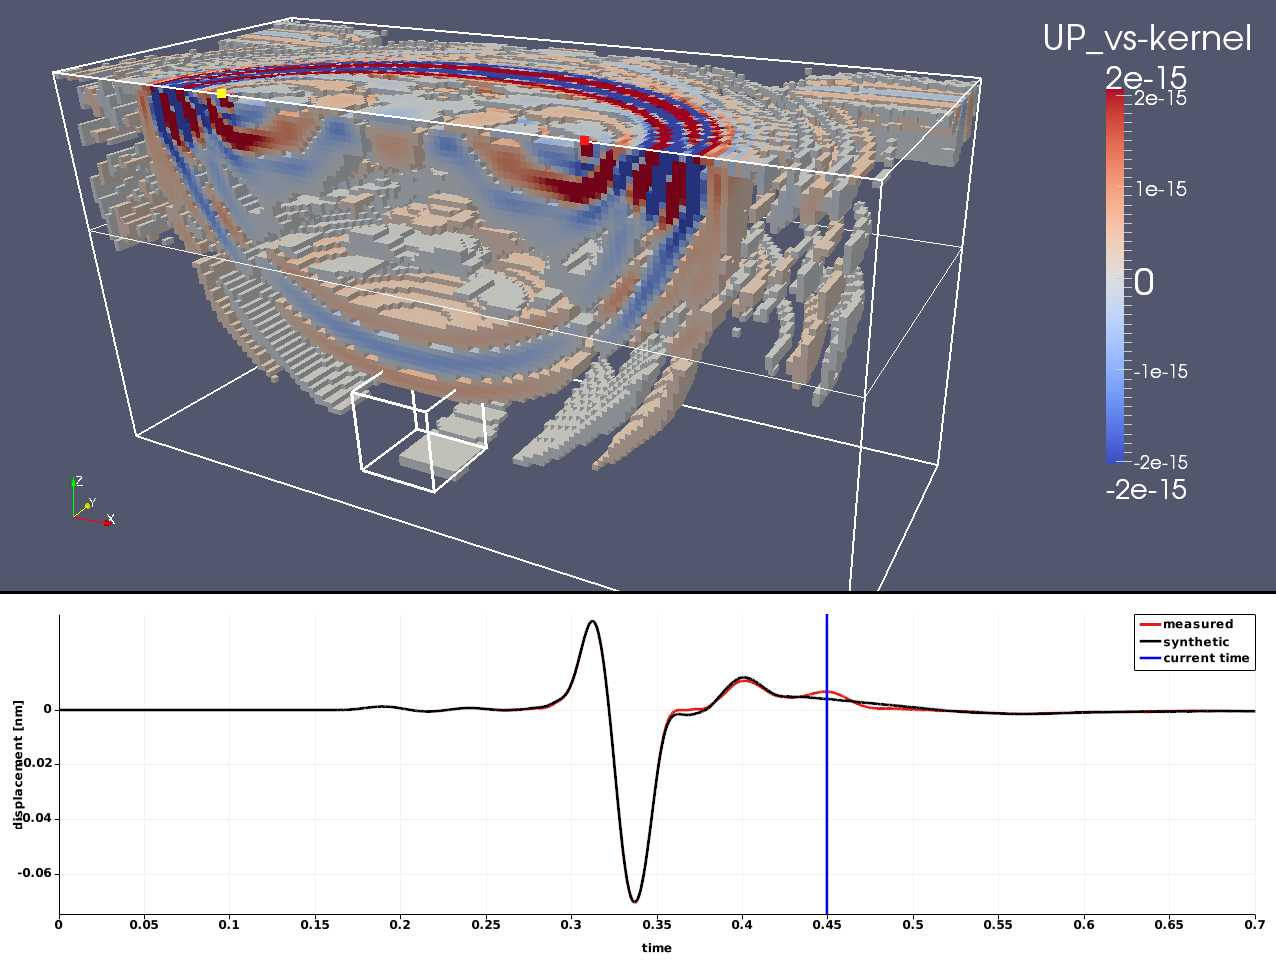
\includegraphics[width=\textwidth]{images/title_time_kernel_analysis.jpg}}
\end{center}

\end{titlepage}
% END individual titlepage
%#########


%
%-------------------------------
% LICENSE
Copyright \copyright 2015 Florian Schumacher.
Permission is granted to copy, distribute and/or modify this document
under the terms of the GNU Free Documentation License, Version 1.3
or any later version published by the Free Software Foundation;
with no Invariant Sections, no Front-Cover Texts, and no Back-Cover Texts.
A copy of the license is included in the section entitled ``GNU
Free Documentation License''.

\vspace{1cm}

If you use \ASKI for your own research, please cite our paper \cite{Schumacher16}:

F. Schumacher, W. Friederich and S. Lamara, \\
"A flexible, extendable, modular and 
computationally efficient approach to scattering-integral-based seismic full waveform 
inversion", \\
\emph{Geophysical Journal International}, \\
Accepted 2015 November 17.  Received 2015 November 17; in original form 2015 April 8\\
http://dx.doi.org/10.1093/gji/ggv505

\vspace{1em}

This documentation was written in the hope that it will be useful to the user,
but it \emph{cannot be assured} that it is accurate in every respect or complete in any sense.
In fact, at some places \emph{this manual is work in progress}.\\
lease do not hesitate to report any inconsistencies via \url{http://www.rub.de/aski} or
to improve this documentation by incorporating your experiences with \ASKI 
and your personal experience of getting used to it (plus, let us know about it! Thanks). 
When you have developed new \ASKI components or 
have modified existing once, please extend / modify this document accoringly.

Furthermore, I am aware of the poor \LaTeX coding of this document. There is a lot of potential
to improve the document 
style, hence the readability of the manual as a whole, as well as the coding style of the 
particular \lcode{.tex} files. \emph{Please do not hesitate to improve!}

The \LaTeX source files and all related components of this document are available via\\
\url{http://www.rub.de/aski}
\begin{flushright}
Florian Schumacher, Dec 2015
\end{flushright}
%
%-------------------------------
% CHAPTER Introduction
\chapter*{How to use this manual}
\phantomsection  % so hyperref creates bookmarks
% -*-LaTex-*-

%-----------------------------------------------------------------------------
%   Copyright 2016 Florian Schumacher (Ruhr-Universitaet Bochum, Germany)
%
%   This file is part of the ASKI manual as a LaTeX document with main file
%   manual.tex
%
%   Permission is granted to copy, distribute and/or modify this document
%   under the terms of the GNU Free Documentation License, Version 1.3
%   or any later version published by the Free Software Foundation;
%   with no Invariant Sections, no Front-Cover Texts, and no Back-Cover Texts.
%   A copy of the license is included in the section entitled ``GNU
%   Free Documentation License''. 
%-----------------------------------------------------------------------------
%
%
%++++++++++++++++++++++++++++++++++++++++++++++++++++++++++
\section*{How to use this manual}
%++++++++++++++++++++++++++++++++++++++++++++++++++++++++++
%
Only chapter~\myref{guide} is intended to be read through, presenting recipes (todo lists/algorithms)
for different workflows that can be conducted by software package \ASKI{}.
For this reason, that chapter is held as compact 
as possible and may itself be regarded as ``the manual'', with the appending chapters only 
containing more specific detail on processes or objects which chapter~\ref{guide} refers to.
After all, the very modular character of \ASKI{} requires documentation which itself is modular.

In other words: just start reading the respective section of chapter~\ref{guide}, which you are interested in 
and whenever you feel the need for more detail follow the respective references. This way, we try to focus
the user on necessary information and successfully guide through the lot of details contained in this document. 

When you conduct a specific \ASKI{} operation for the first time, we recommend you to first fully read through the 
respective guiding list and the referred basic steps before you start running any programs. This way you will 
get an impression of the requirements for your operation.

All chapters appending chapter~\ref{guide} are not intended to be read through section by section but may well
serve the user as a reference. Especially section~\myref{programs_scripts,sec:bin_prog} can provide the 
experienced user with additional executables that conduct some more features which are not referenced somewhere
in the document.

\subsection*{Please preserve your experience!}
If you struggled with the existing \ASKI{} documentation (user manual, comments in code, doxygen, developers 
manual) because it was inconsistent, incomplete or simply wrong and you invested time to find out how it works, 
\emph{please let future generations of users and developers benefit from your gained knowledge!}
Everybody knows that documenting code and writing manuals consumes a lot of time, but correct documentation 
is essential for everyone using and developing software, and I'm sure you know that from your own experience.
So, please invest a bit more time in correcting/extending the \ASKI{} documentation
(where applicable: user manual, comments in code, doxygen, developers manual) and
at best modify the respective source files and issue a pull request on \lcode{gitHub}. In any case let us 
know about it (via \url{https://github.com/seismology-RUB} or \url{http://www.rub.de/aski})!
Otherwise your knowledge is lost forever (you might even lose your knowledge yourself after some while, 
so please write it down).

\emph{Thank you!} (on behalf of everybody)

%
%++++++++++++++++++++++++++++++++++++++++++++++++++++++++++
\section*{Installing \ASKI} %\label{basic_steps,sec:install_ASKI}
%++++++++++++++++++++++++++++++++++++++++++++++++++++++++++
%
\begin{itemize}
\item Clone the latest version of the master branch of the \ASKI{} \lcode{gitHub} repository to some directory 
  (exemplarily called \lcode{/your/programs/}) on your local computer by executing\\
  \lcode{git clone --depth 1 --branch master https://github.com/seismology-RUB/ASKI}\\
  (in one line, of course) from local path \lcode{/your/programs/}~. This will create subdirectory \lcode{/your/programs/ASKI} containing
  the code and documentation of the current release of the \ASKI{} main package.

  Alternatively, go to \url{https://github.com/seismology-RUB/ASKI} and download the content of the master branch
  as a \lcode{.zip} or try executing\\
  \lcode{wget https://github.com/seismology-RUB/ASKI/archive/master.zip}\\
  (in one line, of course) and extract it in such a way that the code files are contained in \lcode{/your/programs/ASKI/}~.

  Webpage \url{http://www.rub.de/aski} might provide additional information for you, just have a look.
\item Follow the directions in file \lcode{ASKI/README.md} for configuration and compilation of the \ASKI{} ececutables.
\end{itemize}
Throughout the \ASKI{} documentation, ``\ASKI{} installation directory'' refers to directory \lcode{ASKI/}, i.e.\
\lcode{/your/programs/ASKI}, where you have cloned/extracted the \lcode{git} repository to.
%
%++++++++++++++++++++++++++++++++++++++++++++++++++++++++++
\section*{Toy example: synthetic waveform inversion}
%++++++++++++++++++++++++++++++++++++++++++++++++++++++++++
%
In order to get familiar with applying \ASKI{} for full waveform inversion, you might consider to 
download and reproduce the synthetic inversion presented in Florian's dissertation 
\cite{_743d334d-dfa4-4a16-8cc5-91cdadc95271} (chapter 5.1) as well as in our GJI paper \cite{Schumacher16} 
(section 4.1), see section~\myref{guide,sec:example_C_borehole}.
%
%++++++++++++++++++++++++++++++++++++++++++++++++++++++++++
\section*{\ASKI{} versions}
%++++++++++++++++++++++++++++++++++++++++++++++++++++++++++
%
\ASKI{}'s release version numbering does not follow any standard of version numbering. 
Since releases were not very frequent so far and the source code was not publically available under version control, 
it was considered sufficient to have only a simple numbering for the purpose of distinguishing release versions.
In case that developments and releases become more frequent in the future, the \ASKI{} developers might consider
to follow some standard for future release version numbering.

\subsection*{\ASKI{} \lcodetitle{0.3}}
\ASKI{}'s first release version was numbered \lcode{0.3}, with \lcode{0} indicating a pre-release
that was not very well tested at that point and \lcode{3} being the third version of internal
development when porting from another internal versioning repository.

\subsection*{\ASKI{} \lcodetitle{1.0}}
After some while of intensive testing and application of \ASKI{} to synthetic and real-world cases, 
as well as development of a lot of \ASKI{} tools, version \lcode{1.0} was released as the first
ready-to-use version of \ASKI{}.

\subsection*{\ASKI{} \lcodetitle{1.1}}
In general, version \lcode{1.1} should be compatible with \lcode{1.0} in terms of file formats and general use
of the software. The main reason for this release was the fix of a pointer problem with \lcode{gfortran}.
Compared with the previous release, some more tools are available (\lcode{addSpikeCheckerToKim}, 
\lcode{createSpectralFilters}, \lcode{create_ASKI_evstat_filters.py}) and forward-code-specific 
definition of complex frequencies is available (e.g. for use with Gemini). Some bugs were fixed.

\subsection*{\ASKI{} \lcodetitle{1.2}}
Version \lcode{1.2} is just an intermediate version number and denotes the status of the code when moving the 
development repository permanently to git and providing the current working ready-to-use version of \ASKI{} by the 
master branch of repository \url{https://github.com/seismology-RUB/ASKI}.

Significant changes to version \lcode{1.1}:
\begin{itemize}
\item 
There is an additional subdirectory \lcode{devel/} containing developer tools and developer documentation.

\item
The source files of the \ASKI{} user manual as well as a compiled pdf of the manual are provided now in subdirectory
\lcode{doc/}

\item 
Inversion grids of type \lcode{chunksInversionGrid} now provide base cell refinement capabilities (at the moment
a random ``toy'' method is implmemented for illustration, but serious refinement method can now be implemented
easily into module \lcode{chunksInversionGrid}.

\item New/renamed/removed tools:

  \lcode{chunksInvgrid2vtk} for special vtk files related to chunks and refined cells 

  \lcode{createShoreLines} (Fortran executable) and \lcode{create_shore_lines.py} (Python program
  utilizing the \lcode{f2py} interface generator) for generating shore line vtk files from native binary GSHHS 
  shore line data files

  Executable \lcode{createMeasuredData} was renamed in \lcode{transformMeasuredData}

  Python script \lcode{create_ASKI_evstat_filters.py} is removed (functionality not required anymore)
\end{itemize}

\subsection*{The \lcodetitle{gitHub} master branch}
After porting \ASKI{} to \url{https://github.com/seismology-RUB/ASKI} in August 2016, the current version of its
master branch should serve as a stable version to use, along with the current versions of the forward code 
packages supported by \ASKI{}.

%
%-------------------------------
% CHAPTER Introduction
\chapter*{What is \ASKI?} \label{guide,sec:ASKI}
\phantomsection  % so hyperref creates bookmarks
% -*-LaTex-*-

%-----------------------------------------------------------------------------
%   Copyright 2016 Florian Schumacher (Ruhr-Universitaet Bochum, Germany)
%
%   This file is part of the ASKI manual as a LaTeX document with main file
%   manual.tex
%
%   Permission is granted to copy, distribute and/or modify this document
%   under the terms of the GNU Free Documentation License, Version 1.3
%   or any later version published by the Free Software Foundation;
%   with no Invariant Sections, no Front-Cover Texts, and no Back-Cover Texts.
%   A copy of the license is included in the section entitled ``GNU
%   Free Documentation License''. 
%-----------------------------------------------------------------------------
%
\ASKI{} is a modularized software package written by the main authors Florian Schumacher and
Wolfgang Friederich (Ruhr-University Bochum, Germany). It offers sensitivity and regularization 
analysis tools for seismic datasets
as well as a scattering-integral-type full waveform inversion (FWI) concept based on waveform sensitivity 
kernels (i.e.\ Fr\'echet derivatives of seismic waveform data functionals) derived from Born scattering theory,
having Gauss-Newton convergence properties.
This inversion concept is presented in our 2016 GJI paper \cite{Schumacher16} and in Florian's doctoral
dissertation \cite{_743d334d-dfa4-4a16-8cc5-91cdadc95271}. The software package \ASKI{} itself is presented
in our 2016 SoftwareX paper \cite{Schumacher16b}.

\ASKI{} does not implement an intrinsic code for simulation of seismic wave propagation in order to 
solve the seismic forward problem, but instead provides generalized interfaces to different external wave 
propagation codes. At the moment, the 1D semi-analytical code Gemini \cite{friederich_wd1995} and the 3D spectral 
element code SPECFEM3D \cite{TrKoLi08} are supported in \emph{both}, Cartesian and spherical framework. 
Additionally \ASKI{} supports the 3D nodal discontinuous Galerkin code NEXD \cite{Lambrecht.2015}
and we plan to implement support for the Finite Difference code SOFI \cite{bohlen2002parallel}
in the future. 
Please do not hesitate to add your own forward code (refer to the \ASKI{} developers manual in
\lcode{devel/doc/ASKI_developers_manual/}). If you encounter any problems or have suggestions to improve this
process, we are happy to hear from you.

The resulting very modular concept of \ASKI{} allows us to keep the spatial description of the inverted 
models completely independent of the spatial description of the model used for solving the forward 
problem. This way, the overall inverse problem can be approached and regularized more physically compared
with using the forward grid for inversion, too. The normally very fine spatial discretization of the model
domain is employed by the forward solver. This discretization is usually weigh too fine to be used
directly for inversion since usually seismic data can only resolve much coarser structures and the
resolving power the data possesses also varies throughout the model domain. 
The separation concept of \ASKI{} \emph{naturally} alows to choose the spatial model
resolution heterogeneously and \emph{anew} in each iteration of FWI.

Instead of using time-dependent values of ground motion (i.e.\ samples of time-serieses of seismic data), 
\ASKI{} uses freqency-dependent complex values of ground displacement, recorded at certain receivers excited 
by certain seismic sources. This, mainly, has reasons of computational feasibility.
For time-domain forward methods, we implement an on-the-fly Fourier Transform in order to provide the
required spectral waveforms. 

Using sensitivity kernels $K$, data residuals $\delta d_i$ are connected to model uptdate values $\delta m_j$ by 
an integral relation $\delta d_i = \int_{\text{Earth}} \delta \vec{m} \cdot \vec{K}_i$. In order to build a linear 
system, the model update $\delta \vec{m}$ is assumed to be constant throughout small scattering volumes 
$\Omega_j$, where $\Omega = \overset{\centerdot}{\bigcup}_j \Omega_j$. These volumes constitute the cells of the volumetric 
inversion grid and the sensitivity matrix contains entries of preintegrated kernels $\int_{\Omega_j} K_i$ (and
model update values $\delta m_j$ are associated with cells $\Omega_j$ for a particular elastic parameter).

The sensitivity kernels $K$ are computed from forward wavefields and strains produced on a set of points in 
space, which
is dependent on the particular forward method. This set of points is refered to in \ASKI{} as 
\emph{wavefield points}. The 
wavefields are written to file, by the respective forward method, which may require large disk space. 
Providing methods for constructing quadrature rules for arbitrary point sets contained in 
arbitrary (hexahedral or tetrahedral) volumes, 
\ASKI{} computes integration weights for integration of functions given on the wavefield points 
(particularly kernels) over the volumetric
cells of the inversion grid. The inversion grid takes care of the localization of wavefield points 
inside the inversion grid cells and, if requested, the transformation of cells to a hexahedral (or tetrahedral) 
standard 
cell for the computation of the integration weights. Hence, exotic combinations of wavefield points (i.e.\ 
forward methods), integration weight types and inversion grid types might not be possible (e.g.\ using the
\lcode{SPECFEM}-internal inversion grid built by the spectral elements along with wavefield points from 
another forward method). 

The pre-integrated kernel values are also written to files, which may be flexibly read in 
(e.g.\ reading in kernels of specific data subsets only)
by the sets of independent \ASKI{} executables conducting any sensitivity analysis 
or interation steps in the iterative full waveform inversion.
Those tools work on the sensitivity matrix, which in the FWI is used in a linear system of equations which
relates data residua $\delta d_i$ to a model improvement $\delta m$. 
In the course of the iterative full waveform inversion, it is naturally possible by \ASKI{} to gradually increase
the frequency content of the inverted data and to choose smaller inversion grid cells in each iteration, 
i.e.\ increasing the spatial resolution dependent on frequency.

%
%-------------------------------
% TABLE OF CONTENTS
\tableofcontents
%
%-------------------------------
% CHAPTER Guide
\setcounter{chapter}{-1}
\chapter{Guide} \label{guide}
%\phantomsection  % so hyperref creates bookmarks
%\addcontentsline{toc}{chapter}{Guide}
% -*-LaTex-*-

%-----------------------------------------------------------------------------
%   Copyright 2016 Florian Schumacher (Ruhr-Universitaet Bochum, Germany)
%
%   This file is part of the ASKI manual as a LaTeX document with main file
%   manual.tex
%
%   Permission is granted to copy, distribute and/or modify this document
%   under the terms of the GNU Free Documentation License, Version 1.3
%   or any later version published by the Free Software Foundation;
%   with no Invariant Sections, no Front-Cover Texts, and no Back-Cover Texts.
%   A copy of the license is included in the section entitled ``GNU
%   Free Documentation License''. 
%-----------------------------------------------------------------------------
%
This chapter is intended to guide you, dependent on what you want to do, through all necessary steps
to achieve your goals.

If you don't know about \ASKI{} yet, we recommend you to quickly read through the previous section 
entitled ``What is \ASKI{}?'', which explains some basic terminology in \ASKI{} and the concepts it is based on.

The sections below address possible operations you can conduct with \ASKI{}. For every operation, we only refer 
to the necessary basic steps (by $\rightarrow$), which are described in chapter~\myref{basic_steps}.\\
Make sure to have a complete read-through before hastily doing anything!

Good Luck!
%
%
%++++++++++++++++++++++++++++++++++++++++++++++++++++++++++
\newpage
\section*{Full Waveform Inversion using pre-integrated spectral Waveform Sensitivity Kernels} \label{guide,sec:classic_inversion}
\phantomsection  % so hyperref creates bookmarks
\addcontentsline{toc}{section}{Full Waveform Inversion - Classical Waveform Sensitivity Kernels}
%++++++++++++++++++++++++++++++++++++++++++++++++++++++++++
%
%
%here short introduction as to what ``Full Waveform Sensitivity Kernel Inversion'' actually is, followed by
%the steps to do:

Iterative inversion scheme which uses waveform sensitivity kernels to gain model updates form data residua.

In addition to \ASKI{} \myaref{basic_steps,sec:install_ASKI}, you will need to install a supported software which 
solves the forward problem \myaref{basic_steps,sec:forward_problem}.
%
%----------------------------------------------------------
\subsection*{Before The First Iteration Step}
%----------------------------------------------------------
%
\begin{itemize}
\item Create a main parameter file (e.g.\ in the parent directory of your specific inversion directory, 
or where you collect main parameter files for all your inversion projects)
\myaref{basic_steps,sec:main_parfile}. You will need this file as an input argument to almost all programs/scripts.\\
Set \lcode{MAIN_PATH_INVERSION} to a correct value. 
The directory does not need to exist yet, if not, then it will be created. \\
You should keep the default values of \lcode{ITERATION_STEP_PATH} and \lcode{PARFILE_ITERATION_STEP} unless
you know what you are doing. If you wish to use different values for the complete inversion process, 
it makes senese to adjust them now.\\
All other parameters can be adjusted later. 
%
\item Create a directory structure for the expected number of iteration steps of your inversion 
\myaref{basic_steps,sec:create_dir}
%
\item Make yourself familiar with the form of data used in \ASKI{} \myaref{basic_steps,sec:data_general}. \\
  Set \lcode{APPLY_EVENT_FILTER}, \lcode{APPLY_STATION_FILTER}, \lcode{PATH_MEASURED_DATA}, 
  \lcode{PATH_EVENT_FILTER}, \lcode{PATH_STATION_FILTER}, 
  \lcode{FILE_EVENT_LIST}, and \lcode{FILE_STATION_LIST}, as well as \lcode{MEASURED_DATA_FREQUENCY_STEP}, 
  \lcode{MEASURED_DATA_NUMBER_OF_FREQ} and \lcode{MEASURED_DATA_INDEX_OF_FREQ}  in your main 
  parameter file, before preparing your data in the required form \myaref{basic_steps,sec:measured_data}, 
  as well as any filters \myaref{basic_steps,sec:filters}.
%
\item Set \lcode{FORWARD_METHOD} in your main 
parameter file to the value of your choice. If you want to use different methods in the course of 
inverting one dataset (e.g.\ starting with a 1D method, continuing with a 3D method), then it may make 
sense to create a different directory structure for each method and using the final model of one method
as the starting model for the next method.
%
\item Choose a model parametrization by setting \lcode{MODEL_PARAMETRIZATION} in the main parameter file 
to a value of your choice (which is supported by your forward method).
%
\end{itemize}
%
%----------------------------------------------------------
\subsection*{Before Each Iteration Step (including the first one)}
%----------------------------------------------------------
%
\begin{itemize}
\item Set \lcode{CURRENT_ITERATION_STEP}
in your main parameter file to the correct value. When continuing your inversion with a different method, you
may also keep the current iteration step index (in order for you not to get confused) and leave 
subdirectories of your \lcode{MAIN_PATH_INVERSION} empty (or delete them after creation if they 
are not needed):\\
e.g.\ an inversion with one method could start with iteration step 4 (and respective subdirectory), 
if you have already conducted 3 iteration steps with other methods.
%
\item Define the inversion grid of the current iteration \myaref{basic_steps,sec:invgrid}.
%
\item Set all parameters in the specific iteration step parameter file to correct values 
\myaref{basic_steps,sec:iter_parfile}, including the correct reference to your inversion grid.
Refer to the documentation of your forward method on how to set filenames \lcode{FILE_WAVEFIELD_POINTS}
and \lcode{FILE_KERNEL_REFERENCE_MODEL} (as the handling of these file are method dependent).
%
\item Dependent on your method and model parametrization, take care about communicating the current
model (inverted in the previous iteration) to your forward method \myaref{basic_steps,sec:export_kim}. 
Before the first iteration, however, you need to define some starting model \myaref{basic_steps,sec:start_model}.
%
\end{itemize}
%
%----------------------------------------------------------
\subsection*{Conducting An Iteration Step}
%----------------------------------------------------------
%
\begin{itemize}
\item Compute forward wavefields and Green tensor components w.r.t.\ the current model 
by your method. Refer to the respective documentation of your method.\\
After that, you may prepare the synthetic data in the way \ASKI{} expects it (see sections~\myref{basic_steps,sec:data_general} 
and~\myref{files,sec:synth_data}). Refer to the documentation of your method on how to do it.
%
\item Set \lcode{TYPE_INTEGRATION_WEIGHTS} in the iteration specific parameter file 
\myaref{basic_steps,sec:intw}.
You should keep the default values of \lcode{FILE_INTEGRATION_WEIGHTS},
unless you know what you are doing (can be any name, will be created, but is referred to, afterwards. 
You could compute different types of weights and store them in different files, this way). 
%
\item Initiate basic requirements for all programs and scripts \myaref{basic_steps,sec:initBasics}.
%
\item Define data and model space, where the paths are mainly important for now \myaref{basic_steps,sec:dmspace}.
%
\item Compute sensitivity kernels for your specific set of paths and your set of model parameters 
  \myaref{basic_steps,sec:compute_kernels}. \\
  If desired, you may have a look at your kernels \myaref{basic_steps,sec:plot_kernels}.
%
\item Choose a specific data and model space. You may well play around with different subsets of data or
smoothing (next step) in the course of inverting for different models \myaref{basic_steps,sec:dmspace}.
%
\item Finally compute the inverted model by solving the kernel system \myaref{basic_steps,sec:solve_kernel_system},
  possibly varying the regularization constraints.
%
\item After deciding whether or not to do another iteration of full waveform inversion and choosing a model 
  for the next iteration \myaref{basic_steps,sec:investigate_convergence}, repeat all operations beginning 
  with ``Before Each Iteration Step (including the first one)''.
\end{itemize}
%
%++++++++++++++++++++++++++++++++++++++++++++++++++++++++++
\newpage
\section*{Cross Borehole Example} \label{guide,sec:example_C_borehole}
\phantomsection  % so hyperref creates bookmarks
\addcontentsline{toc}{section}{Cross Borehole Example}
%++++++++++++++++++++++++++++++++++++++++++++++++++++++++++
%
This section describes the synthetic cross borehole example presented in Florian's dissertation 
\cite{_743d334d-dfa4-4a16-8cc5-91cdadc95271} (chapter 5.1) as well as in our GJI paper \cite{Schumacher16} 
(section 4.1). It is an example of lull waveform inversion using pre-integrated spectral waveform sensitivity 
kernels (as described in the first recipe of this chapter Guide (page~\pageref{guide}).

The example files referred to in the following, were computed with \ASKI{} version 1.0, which however should
not pose any problem since the changed from version 1.0 to 1.1 do not effect the computations or compatibility
of any output files. It may, however, 
occur that numbers might not be reproduced in a numerically equal way, which is also likely to happen
when a different compiler (version) is used. 

Install \ASKI{} \myaref{basic_steps,sec:install_ASKI}. 

Then download the example
files \lcode{ASKI_inversion_cross_borehole.tar.gz} via \url{http://www.rub.de/aski} (566 MB). 
In this package, all files of the first 2 iterations (plus illustrating extras) are provided. 
In order to keep the download small, wavefield output is not provided  for
iterations 3 to 12. You should be able to reproduce the wavefields immendiately for any iteration step
from the provided inverted models without reproducing all preceeding iterations. 
The pre-integrated sensitivity kernel files are only provided for
iterations 1 to 3. Kernel files for the other iterations can be downloaded by
interested users seperately via \url{http://www.rub.de/aski} (package\\
\lcode{ASKI_inversion_cross_borehole_sensitivity_kernels_iter04-iter12.tar.gz}, (907 MB).

\emph{Most importantly}, you must change the value of \lcode{MAIN_PATH_INVERSION}
in file\\
\lcode{ASKI_inversion_cross_borehole/main_parfile_cross_borehole} to
\lcode{"your_base_path/"} in order for all the example directory to work. 
If you do not want to overwrite the existing output, alternatively you 
should create a separate inversion directory from scratch~\myaref{basic_steps,sec:create_dir}
 and leave \lcode{ASKI_inversion_cross_borehole/}
as a reference only. 

This example was generated using \lcode{SPECFEM3D_Cartesian 3.0} for \ASKI{}. Even if you intend
to use a different forward method, you can still practice the operations of the main \ASKI{}
package and, thus, learn about how to conduct any steps in
the full waveform inversion \emph{after} the forward problem is solved. Just read the description
of the contained files in \\
\lcode{ASKI_inversion_cross_borehole/README}.

If you want to reproduce also the forward wavefields from \lcode{SPECFEM3D_Cartesian 3.0}, 
you need to install it, of course~\myaref{basic_steps,sec:forward_problem}.
%
%
%++++++++++++++++++++++++++++++++++++++++++++++++++++++++++
\newpage
\section*{Time-Domain Sensitivity Kernels} \label{guide,sec:time_kernels}
\phantomsection  % so hyperref creates bookmarks
\addcontentsline{toc}{section}{Time-Domain Sensitivity Kernels}
%++++++++++++++++++++++++++++++++++++++++++++++++++++++++++
%
%
This section describes, how to compute time-domain waveform sensitivity kernels for a specific set 
of sources receivers with respect to a certain background earth model as an operation seperate of any
other \ASKI{} operations. The kernels in time-domain are much more intuitive to look at for human beings, 
than the standard frequency-domain sensitivity kernels. You may, as well, compute time-domain sensitivity 
kernels from the kernels produced in any iteration step of a full waveform inversion 
(page \pageref{guide,sec:classic_inversion}). For this purpose, apply the steps 
``Transforming to Time-Domain Sensitivity Kernels'' (below) after you computed the spectral kernels in 
you iteration step, as the time-domain waveform kernels are produced by an inverse Fourier transform 
from the standard frequency-domain waveform sensitivity kernels on which \ASKI{} is based.

Please do not get confused by the general terminology of \emph{inversion} and \emph{iteration}, etc. 
Technically you will be conducting an incomplete first iteration step of a full waveform inversion, 
using all the program infrastructure which is also used for a full waveform inversion. 

In addition to \ASKI{} \myaref{basic_steps,sec:install_ASKI}, you will need to install a supported software which 
solves the forward problem \myaref{basic_steps,sec:forward_problem}.
%
%----------------------------------------------------------
\subsection*{Preceding Considerations}
%----------------------------------------------------------
%
\begin{itemize}
\item Create a main parameter file (e.g.\ in the parent directory of your specific inversion directory, 
or where you collect main parameter files for all your inversion projects or analyses)
\myaref{basic_steps,sec:main_parfile}. You will need this file as an input argument to almost all programs/scripts.\\
Set \lcode{MAIN_PATH_INVERSION} to a correct value.
The directory does not need to exist yet, if not, then it will be created. \\
Set \lcode{ITERATION_STEP_PATH} and 
\lcode{PARFILE_ITERATION_STEP} to desired values, 
or leave the default values, if present.\\
All other parameters can be adjusted later. 
%
\item Create a directory structure for only one iteration step \myaref{basic_steps,sec:create_dir}
%
\item Even if you do not have any measured data, it might still be beneficial for you to make yourself 
(roughly) familiar with the form of data used in \ASKI{} \myaref{basic_steps,sec:data_general}. \\
In your main parameter file, set the following values: 
  \begin{itemize}
  \item Set \lcode{FILE_EVENT_LIST} and \lcode{FILE_STATION_LIST} to define the sources and receivers which are
    involved in the paths that you would like to compute the kernels for. 
  \item Dependent on the (length of the) time series you want to deal with, define the frequency discretization of the
    spectral kernels that will be produced first. This must be done by \lcode{MEASURED_DATA_FREQUENCY_STEP}, 
    \lcode{MEASURED_DATA_NUMBER_OF_FREQ} and \lcode{MEASURED_DATA_INDEX_OF_FREQ}.
  \end{itemize}
In general, for the pure kernel computation you do not need any measured data. So, here you do not need to prepare
data in the \ASKI{} required form.
%
\item Set \lcode{APPLY_EVENT_FILTER}, \lcode{APPLY_STATION_FILTER} (and if required \lcode{PATH_EVENT_FILTER} and 
  \lcode{PATH_STATION_FILTER}) in your main parameter file. In case the forward wavefields were calculated w.r.t.\ an
  impulse source time function (or the source-time function was deconvolved), you should apply filters 
  \myaref{basic_steps,sec:filters} that taper down the amplitude spectrum before the maximum frequency used. 
  Otherwise, the inverse Fourier transform below can create artefacts.
%
\item Set \lcode{FORWARD_METHOD} in your main parameter file to the value of your choice. 
%
\item Choose a model parametrization by setting \lcode{MODEL_PARAMETRIZATION} in the main parameter file 
to a value of your choice (which is supported by your forward method).
%
\item Set \lcode{CURRENT_ITERATION_STEP} in your main parameter file to value \lcode{1}, as you are technically
starting to conduct the first (and only) iteration step of a full waveform inversion.
%
\item It is highly recommended to set \lcode{DEFAULT_VTK_FILE_FORMAT} to \lcode{BINARY} in the main parameter file, 
  since a lot of \lcode{vtk} files might be generated (one for every time step). Using the binary format significantly
  reduces storage.

\item Define the inversion grid \myaref{basic_steps,sec:invgrid}, which controls the spacial volumetric discretization 
(resolution) of the computed sensitivity kernels. In case of just computing (time) kernels to look at, it is not
crucial to regard this resolution as the resolution of some inverted model, as no inversion will be conducted on the 
inversion grid. Since there might be a lot of \lcode{vtk} files generated (one for every time step), it is highly recommended to set\\
\lcode{VTK_GEOMETRY_TYPE = CELL_CENTERS} in the inversion grid parameter file (if your type of inversion grid
supports that functionality). This significantly reduces the amount of geometry information written to the 
\lcode{vtk} files, hence their size.
%
\item Set all parameters in the specific iteration step parameter file to correct values 
\myaref{basic_steps,sec:iter_parfile}, including the correct reference to the inversion grid. Set 
\lcode{ITERATION_STEP_NUMBER_OF_FREQ} and \lcode{ITERATION_STEP_INDEX_OF_FREQ} to the \emph{same} values as the
\lcode{MEASURED_DATA_NUMBER_OF_FREQ} and \lcode{MEASURED_DATA_INDEX_OF_FREQ} in the main parameter file!
Refer to the documentation of your forward method on how to set filenames \lcode{FILE_WAVEFIELD_POINTS}
and \lcode{FILE_KERNEL_REFERENCE_MODEL} (as the handling of these file are method dependent).
%
\item Dependent on your method and model parametrization, define your background model with respect to which the
kernels will be computed. If you have some inverted model file, use \myaref{basic_steps,sec:export_kim}. For defining
a starting model, see \myaref{basic_steps,sec:start_model}.
%
\end{itemize}
%
%----------------------------------------------------------
\subsection*{Computing Spectral Waveform Sensitivity Kernels}
%----------------------------------------------------------
%
\begin{itemize}
\item Compute forward wavefields and Green tensor components w.r.t.\ the current model 
by your method. Refer to the respective documentation of your method.\\
After that, you may prepare the synthetic data in the way \ASKI{} expects it (see sections~\myref{basic_steps,sec:data_general} 
and~\myref{files,sec:synth_data}). Refer to the documentation of your method on how to do it.
%
\item Set \lcode{TYPE_INTEGRATION_WEIGHTS} in the iteration specific parameter file 
\myaref{basic_steps,sec:intw}. If you intend to compute the time kernels on wavefield points only, you will technically
never use the integration weights, but nevertheless they need to be correctly created (in that case use a simple
type of weights like 5 or 0).
You should keep the default values of \lcode{FILE_INTEGRATION_WEIGHTS},
unless you know what you are doing (can be any name, will be created, but is referred to, afterwards. 
You could compute different types of weights and store them in different files, this way). 
%
\item Initiate basic requirements for all programs and scripts \myaref{basic_steps,sec:initBasics}.
%
\item If you have many paths, you may define a data and model space concentrating on defining paths 
  \myaref{basic_steps,sec:dmspace}.
  If you have only one path or just a few, it is possible (and propably also convenient) to just continue to the
  computation of the kernels.
%
\item Compute the standard frequency-domain sensitivity kernels for your specific set of paths (or the one or 
  few paths, one after another). In case you want to transform to time-domain kernels \emph{on wavefield points} 
  (and not pre-integrated kernels on inversion grid),
  use option \lcode{-wp} \myaref{basic_steps,sec:compute_kernels} \\
  If desired, you may have a look at the standard frequency-domain kernels \myaref{basic_steps,sec:plot_kernels}.
\end{itemize}
%
%----------------------------------------------------------
\subsection*{Transforming to Time-Domain Sensitivity Kernels}
%----------------------------------------------------------
%
\begin{itemize}
\item Transform the standard frequency-domain waveform kernels to time domain. In case you want to get  
  time-domain kernels \emph{on wavefield points}, (and not pre-integrated kernels on inversion grid),
  you must use option \lcode{-wp} (in this case, you already should have used \lcode{-wp} to compute 
  spectral kernels) \myaref{basic_steps,sec:compute_time_kernels}.\\
  Make sure that the wavefield spectra have a sufficiently small amplitude spectrum at high frequencies, in order for the
  inverse Fourier Transform to work satisfactorily. Otherwise use filters.
%
\item Plot the time kernels \myaref{basic_steps,sec:plot_time_kernels}.
\end{itemize}
%
%++++++++++++++++++++++++++++++++++++++++++++++++++++++++++
\newpage
\section*{Analysis of Acquisition Geometry using Kernel Focussing} \label{guide,sec:acq_ana_focus}
\phantomsection
\addcontentsline{toc}{section}{Analysis of Acquisition Geometry using Kernel Focussing}
%++++++++++++++++++++++++++++++++++++++++++++++++++++++++++
%
{\bf THIS SECTION IS WORK IN PROGRESS!}

%Short introduction as to what ``Analysis of Acquisition Geometry using Kernel Focussing'' actually is:
The general concept of Backus-Gilbert-based focussing of sensitivity kernels on a defined focussing region 
in the model space is published in \cite{_743d334d-dfa4-4a16-8cc5-91cdadc95271}, Chapter 7.1. On the basis
of this way of finding linear combinations of data which are sensitive only to changes in a model subspace, 
the dataset can be analysed w.r.t.\ finding event-station paths (and components / frequencies) which optimally
illuminate the model subspace. 

Executable \lcode{focusSpectralKernels} \myaref{programs_scripts,sec:bin_prog,sec:focus_spec_kernel} produces the coefficients of the linear combination of data required
for the analysis. However, this section does not yet give a detailed list of steps how to conduct such 
an analysis. 

\begin{itemize}
\item step 1
\item step 2
\item ...
\end{itemize}
%
%++++++++++++++++++++++++++++++++++++++++++++++++++++++++++
\newpage
\section*{Full Waveform Inversion - Focused Waveform Sensitivity Kernels} \label{guide,sec:focused_inversion}
\phantomsection
\addcontentsline{toc}{section}{Full Waveform Inversion - Focused Waveform Sensitivity Kernels}
%++++++++++++++++++++++++++++++++++++++++++++++++++++++++++
%
{\bf THIS SECTION IS WORK IN PROGRESS!}

%Short introduction as to what ``Full Waveform Inversion using Focused Data for Maximum Resolution'' actually is:
The general concept of Backus-Gilbert-based focussing of sensitivity kernels on a defined focussing region 
in the model space is published in \cite{_743d334d-dfa4-4a16-8cc5-91cdadc95271}, Chapter 7.1. On the basis
of this way of finding linear combinations of data which are sensitive only to changes in a model subspace, 
different disjoint subdivisions of the model space can be chosen, finding the finest subdivision that
is resolved by the data (i.e.\ where focussing of sensitivity on each subdivision cell is still successfull).
This gives the finest model space that the data can resolve. Also this gives a set of ``new'' data consisting of
linear combinations of the original data, for which each of this new data is sensitive only to a certain
spot in the model space. Doing inversion steps of full waveform inversion with the focussed kernels and the 
focussed data, the hope is to overall conduct a waveform inversion at the maximum resolving power of the data. 
This can also be seen as a sophisticated form of regularizing the overall inverse problem. 

Such a ``focussed waveform inversion'' still remains an idea and was not yet approached to be implemented
in \ASKI{}. Please don't hesitate to implement and test this concept.

todo list:
\begin{itemize}
\item step 1
\item step 2
\item ...
\end{itemize}


%
%-------------------------------
% CHAPTER Basic Steps
%\setcounter{chapter}{-1}
\chapter{Basic Steps} \label{basic_steps}
%-----------------------------------------------------------------------------
%   Copyright 2013 Florian Schumacher
%
%   This file is part of the ASKI manual as a LaTeX document with main file
%   manual.tex
%
%   Permission is granted to copy, distribute and/or modify this document
%   under the terms of the GNU Free Documentation License, Version 1.3
%   or any later version published by the Free Software Foundation;
%   with no Invariant Sections, no Front-Cover Texts, and no Back-Cover Texts.
%   A copy of the license is included in the section entitled ``GNU
%   Free Documentation License''. 
%-----------------------------------------------------------------------------
%
In general, in this chapter we provide only basic information. For more detail on 
specific steps or objects, we always refer to the respective sections below in this document.
%
%++++++++++++++++++++++++++++++++++++++++++++++++++++++++++
\section{Installing \ASKI} \label{basic_steps,sec:install_ASKI}
%++++++++++++++++++++++++++++++++++++++++++++++++++++++++++
%
\begin{itemize}
\item Download here: \url{http://www.rub.de/ASKI}
\item Unpack tar ball somewhere
\item Follow the directions in file \lcode{ASKI_0.3/README}
\end{itemize}
%
%++++++++++++++++++++++++++++++++++++++++++++++++++++++++++
\section{Create Main Parameter File} \label{basic_steps,sec:main_parfile}
%++++++++++++++++++++++++++++++++++++++++++++++++++++++++++
%
The simplest way to create a specific main parameter file for your operation is to modify / adjust 
a copy of the template file \lcode{template/main_parfile_template}. 

Refer to the commented documentation in \lcode{main_parfile_template} or 
to sections~\myref{files,sec:parfiles} and~\myref{files,sec:main_parfile}.
%
%++++++++++++++++++++++++++++++++++++++++++++++++++++++++++
\section{Iteration Step Parameter Files} \label{basic_steps,sec:iter_parfile}
%++++++++++++++++++++++++++++++++++++++++++++++++++++++++++
%
Having created a directory environment for your operation, as described in section~\myref{basic_steps,sec:create_dir},
there should automatically have been created template
parameter files in each directory of an iteration step, having filenames as defined by
parameter \lcode{PARFILE_ITERATION_STEP} in the main parameter file.

Refer to the commented documentation in those template files or 
to sections~\myref{files,sec:parfiles} and~\myref{files,sec:iter_parfile}.
%
%++++++++++++++++++++++++++++++++++++++++++++++++++++++++++
\section{Create Directory Environment} \label{basic_steps,sec:create_dir}
%++++++++++++++++++++++++++++++++++++++++++++++++++++++++++
%
Call python script \lcode{create_ASKI_dir.py}
\begin{lstlisting}
USAGE: please give 2 arguments:
[1] main parmeter file of inversion
[2] number of iteration steps

EXAMPLE:
create_ASKI_dir.py ./main_parfile_Aegean1 10
\end{lstlisting}
Put your main parameter file (see~\myref{basic_steps,sec:main_parfile}) as the first, and the expected 
number of iteration steps as the second argument. \\
You can always \emph{recall this script at any later time} with a larger number of iteration steps. 
All existing directories \emph{will not be affected}, only additional non-existing objects will be 
created. Recalling this script with a smaller number of steps will not delete anything.
%
%++++++++++++++++++++++++++++++++++++++++++++++++++++++++++
\section{Data in \ASKI} \label{basic_steps,sec:data_general}
%++++++++++++++++++++++++++++++++++++++++++++++++++++++++++
%
One certain data sample in \ASKI is characterized by a seismic \emph{source}, a \emph{component} 
of a seismic \emph{receiver}, and a \emph{frequency}, as well as if it is \emph{real} or \emph{imaginary} part 
of the complex spectral values. It has the value of displacement of the ground in the unit of meters.
%
%----------------------------------------------------------
\subsection*{Events and Receivers}
%----------------------------------------------------------
%
The events file (\myref{files,sec:event_list}) and stations file (\myref{files,sec:station_list}) constitute a
collection of \emph{all} events (stations) which will be involved \emph{in any way} in your \ASKI operation.\\
All programs/scripts will refer to a specific event (station) by its event-ID (station-name).
%
%----------------------------------------------------------
\subsection*{Receiver Components}
%----------------------------------------------------------
%
All programs/scripts will refer to a specific receiver component by the following abbreviatory names.\\
Dependent on the coordinate system in which the receivers are defined (Cartesian or spherical, which is 
defined by the first line of the station list file), the supported names of receiver components may have a 
different meaning:
\subsubsection{Cartesian receivers}
\begin{itemize}
\item[] \lcode{CX}: Cartesian \lcode{X}-coordinate (first Cartesian coordinate)
\item[] \lcode{CY}: Cartesian \lcode{Y}-coordinate (second Cartesian coordinate)
\item[] \lcode{CZ}: Cartesian \lcode{Z}-coordinate (third Cartesian coordinate)
\item[] \lcode{N}: same as \lcode{-CX}
\item[] \lcode{S}: same as \lcode{CX}
\item[] \lcode{E}: same as \lcode{CY}
\item[] \lcode{W}: same as \lcode{-CY}
\item[] \lcode{UP}: same as \lcode{CZ}
\item[] \lcode{DOWN}: same as \lcode{-CZ}
\end{itemize}
\subsubsection{Spherical receivers}
\begin{itemize}
\item[] \lcode{CX}: Cartesian \lcode{X}-coordinate with \lcode{X}-axis through equator and $0^\circ$-meridian
\item[] \lcode{CY}: Cartesian \lcode{Y}-coordinate with \lcode{Y}-axis through equator and $90^\circ$E-meridian
\item[] \lcode{CZ}: Cartesian \lcode{Z}-coordinate with \lcode{Z}-axis through north pole
\item[] \lcode{N}: local north
\item[] \lcode{S}: local south
\item[] \lcode{E}: local east
\item[] \lcode{W}: local west
\item[] \lcode{UP}: local up
\item[] \lcode{DOWN}: local down
\end{itemize}
%
%----------------------------------------------------------
\subsection*{Frequency Discretization}
%----------------------------------------------------------
%
In \ASKI, frequencies are given by a frequency step $\Delta f$[Hz] and by a set of integer valued 
frequency indices.

For specific frequency index $i$, the corresponding frequency $f_i$ [Hz] computes as $f_i \,=\, i \,\cdot\, \Delta f$.
E.g.\ $\Delta f \,=\, 10$ Hz and frequency indices $i \,=\, 2,\; 3,\; 5,\; 7,\; 10$ define the set of 
discrete frequencies $f_i \,=\, 20.0,\; 30.0,\; 50.0,\; 70.0,\; 100.0$ [Hz].
%
%++++++++++++++++++++++++++++++++++++++++++++++++++++++++++
\section{Prepare Measured Data} \label{basic_steps,sec:measured_data}
%++++++++++++++++++++++++++++++++++++++++++++++++++++++++++
%
{\bf In the future}, we plan to have a binary program \lcode{createMeasuredData}, which converts time-domain data 
to the special frequency-domain form required by \ASKI. It is planned to supporte measured data given in some 
basic data formats like Seismic Unix and time-series given as textfiles per trace.

For now, you must prepare measured data files on your own as required by \ASKI, see sections~\myref{basic_steps,sec:data_general} 
and~\myref{files,sec:measured_data}. 
%
%++++++++++++++++++++++++++++++++++++++++++++++++++++++++++
\section{Define an Inversion Grid} \label{basic_steps,sec:invgrid}
%++++++++++++++++++++++++++++++++++++++++++++++++++++++++++
%
There are different types of \ASKI inversion grids suitable for different geometries, 
forward methods, hence, applications.

All inversion grids are defined by setting parameters \lcode{TYPE_INVERSION_GRID} and 
\lcode{PARFILE_INVERSION_GRID} in the parameter file of the current iteration step.

In the following, we present the supported inversion grid types and explain the particular
parameters in the respective inversion grid parameter file.
%
%----------------------------------------------------------
\subsection{\lcodetitle{scartInversionGrid}} \label{basic_steps,sec:invgrid,sub:scart}
%----------------------------------------------------------
%
A \lcode{S}imple \lcode{CART}esian inversion grid covers a Cartesian cuboid which can
be shifted to a certain location in Cartesian space and may be rotated about the local vertical
axis. Its cells are distributed in layers. Each layer has a certain thickness and a regularly
distributed number of inversion grid cells along each lateral direction of the cuboid.

Please consult the documentation of your forward method (\myref{basic_steps,sec:forward_problem}) if it supports
inversion grids of type \lcode{scartInversionGrid}. \\
All coordinates, e.g.\ of events and stations or wavefield points, are interpreted by this type of inversion grid as
\lcode{X} (first coordinate), \lcode{Y} (second coordinate), \lcode{Z} (third coordinate). Their
units (e.g.\ meters or kilometers) are not assumed by the inversion grid and are essentially defined by the wavefield
points, hence, they might be method dependent and must be overall consistend.\\
Every type of integration weights is supported by this type of inversion grid, except weights of type 
\lcode{6} (external integration weights).

\begin{figure}[ht]
  \centering
  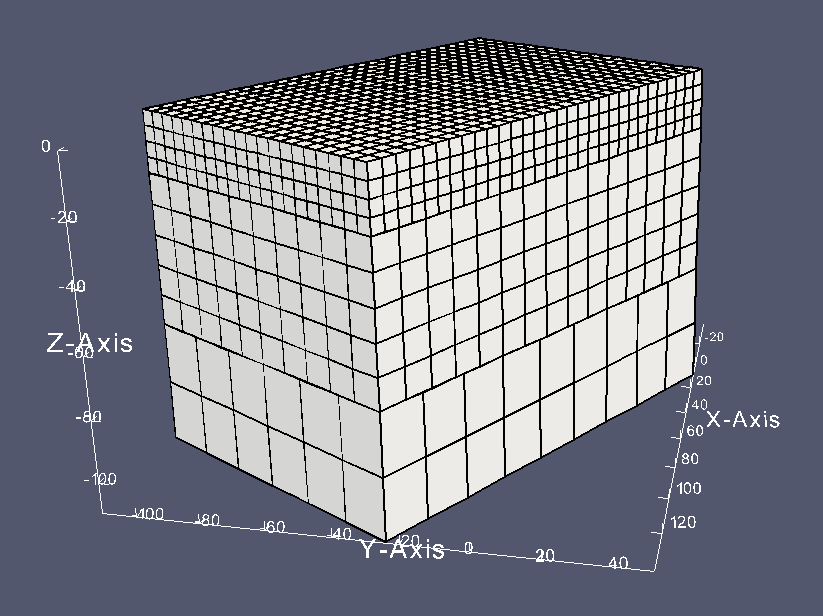
\includegraphics[width=0.5\textwidth]{images/scartInversionGrid_manual.png}
  \caption{Example of a simple Cartesian inversion grid}
  \label{basic_steps,sec:invgrid,sub:scart,fig:grid}
\end{figure}

The shape of the cuboid, as well as the distribution of inversion grid cells, are defined 
via a paramter file, a template of which is file \lcode{template/scartInversionGrid_parfile_template}.
In the following, the particular parameters are explained, with the example
values always refering to the inversion grid as displayed in figure~\myref{basic_steps,sec:invgrid,sub:scart,fig:grid}.

%- - - - - - - - - - - - - - - - - - - - - - - - - - - - - 
\subsubsection{\lcode{SCART_INVGRID_CX}}
\lcode{X}-coordinate of center of cuboid (real number)\\
Example:\\
\lcode{SCART_INVGRID_CX = 50.0}
%- - - - - - - - - - - - - - - - - - - - - - - - - - - - - 
\subsubsection{\lcode{SCART_INVGRID_CY}}
\lcode{Y}-coordinate of center of cuboid (real number)\\
Example:\\
\lcode{SCART_INVGRID_CY = -30.0}
%- - - - - - - - - - - - - - - - - - - - - - - - - - - - - 
\subsubsection{\lcode{SCART_INVGRID_ZMAX}}
Maximum \lcode{Z}-coordinate of cuboid (real number), i.e.\ \lcode{Z}-coordinate of the 
``surface'' of the inversion grid\\
Example:\\
\lcode{SCART_INVGRID_ZMAX = 0.0}
%- - - - - - - - - - - - - - - - - - - - - - - - - - - - - 
\subsubsection{\lcode{SCART_INVGRID_WX}}
Width of cuboid in \lcode{X}-direction (real number)\\
Example:\\
\lcode{SCART_INVGRID_WX = 100.0}
%- - - - - - - - - - - - - - - - - - - - - - - - - - - - - 
\subsubsection{\lcode{SCART_INVGRID_WY}}
Width of cuboid in \lcode{Y}-direction (real number)\\
Example:\\
\lcode{SCART_INVGRID_WY = 150.0}
%- - - - - - - - - - - - - - - - - - - - - - - - - - - - - 
\subsubsection{\lcode{SCART_INVGRID_ROT}}
Angle in degrees of anti-clockwise rotation about the local \lcode{Z}-axis through the 
lateral center of the cuboid (real number)\\
Example:\\
\lcode{SCART_INVGRID_ROT = 60.0}
%- - - - - - - - - - - - - - - - - - - - - - - - - - - - - 
\subsubsection{\lcode{SCART_INVGRID_NREF_BLOCKS,SCART_INVGRID_NLAY,SCART_INVGRID_THICKNESS}}
For an arbitrary number of \lcode{SCART_INVGRID_NREF_BLOCKS} blocks of layers,
the vectors \lcode{SCART_INVGRID_NLAY} (integer values) and \lcode{SCART_INVGRID_THICKNESS} (real values), 
both of length \lcode{SCART_INVGRID_NREF_BLOCKS}, define the \lcode{Z}-direction refinement of each block,
whereby \lcode{SCART_INVGRID_NLAY(i)} defines the number of layers in block \lcode{i}, and 
\lcode{SCART_INVGRID_THICKNESS(i)} defines the thickness of all layers contained in block \lcode{i}.\\
Hence, the overall \lcode{Z}-direction coverage of the inversion grid is defined by 
\lcode{SCART_INVGRID_ZMAX} (which is the coordinate of the top of the first layer in the first refinement block)
and \lcode{SCART_INVGRID_ZMAX - SUM_i(THICKNESS(i) * NLAY(i))} (coordinate of the bottom of the last layer in
%and \lstinline[breaklines=true]$SCART_INVGRID_ZMAX - SUM_i(THICKNESS(i) * NLAY(i))$ (coordinate of the bottom of the last layer in
%and \nolinkurl{SCART_INVGRID_ZMAX - SUM_i(THICKNESS(i) * NLAY(i))} (coordinate of the bottom of the last layer in
last refinement block).\\
Example:\\
\lcode{SCART_INVGRID_NREF_BLOCKS =  3}\\
\lcode{SCART_INVGRID_NLAY =  4   5   2}\\
\lcode{SCART_INVGRID_THICKNESS =  5.0  10.0  20.0}
%- - - - - - - - - - - - - - - - - - - - - - - - - - - - - 
\subsubsection{\lcode{SCART_INVGRID_NX}}
Vector (of length \lcode{SCART_INVGRID_NREF_BLOCKS}) of integer values, defining number of 
inversion grid cells in \lcode{X}-direction, one value for each refinement block\\
Example:\\
\lcode{SCART_INVGRID_NX = 20 10 6}
%- - - - - - - - - - - - - - - - - - - - - - - - - - - - - 
\subsubsection{\lcode{SCART_INVGRID_NY}}
Vector (of length \lcode{SCART_INVGRID_NREF_BLOCKS}) of integer values, defining number of 
inversion grid cells in \lcode{Y}-direction, one value for each refinement block\\
Example:\\
\lcode{SCART_INVGRID_NX = 30 15 9}
%- - - - - - - - - - - - - - - - - - - - - - - - - - - - - 
\subsubsection{\lcode{USE_LOCAL_INVGRID_COORDS_FOR_VTK}}
Logical value to indicate whether to use local inversion grid coordinates for vtk geometry, i.e.\ no rotation 
by \lcode{SCART_INVGRID_ROT} and no shift by \lcode{SCART_INVGRID_CX}, \lcode{SCART_INVGRID_CY}, 
\lcode{SCART_INVGRID_ZMAX} (cuboid centered in \lcode{X=Y=0} and \lcode{ZMAX=0})\\
Example:\\
\lcode{USE_LOCAL_INVGRID_COORDS_FOR_VTK = .false.}
%- - - - - - - - - - - - - - - - - - - - - - - - - - - - - 
\subsubsection{\lcode{SCALE_VTK_COORDS,VTK_COORDS_SCALING_FACTOR}}
Scale vtk geometry coordinates by factor \lcode{VTK_COORDS_SCALING_FACTOR} (real number), if 
\lcode{SCALE_VTK_COORDS = .true.}. This may be helpful if coordinate values (e.g.\ in meters) 
get so large that they cause problems when plotting in paraview.\\
Example:\\
\lcode{SCALE_VTK_COORDS = .false.}\\
\lcode{VTK_COORDS_SCALING_FACTOR = 1.0}
%- - - - - - - - - - - - - - - - - - - - - - - - - - - - - 
%
%----------------------------------------------------------
\subsection{\lcodetitle{ecartInversionGrid}} \label{basic_steps,sec:invgrid,sub:ecart}
%----------------------------------------------------------
%
{\bf WARNING, EXPERIMENTAL FEATURE:} \emph{so far, this type of inversion grid works for tetrahedral cells only,
since support for hexahedreal cells is not completed throughout. However, even for tetrahedra the automatic detection 
of neighbours did not work properly in some test cases! So if you intend to use this inversion grid, please have a look 
at the grid and all neighbours (neighbours only required for model smoothing in case of solving the Kernel system of equations).
You can do that by using binary program} \lcode{invgrid2vtk} \emph{along with option} \lcode{-nb} \emph{. Call} 
\lcode{invgrid2vtk -h} \emph{for further details on how to use it.}

An \lcode{E}xternal \lcode{CART}esian inversion grid is defined by several text files containing the definintion 
of nodes (i.e.\  essentially the corner points, or rather the control nodes of the inversion grid cells) and the 
definition of cells by refering to the nodes. At the moment, 4-node tetrahedral cells are fully supported, and 8-node 
hexahedral cells are partly supported. 
Those files may be produced by any meshing tool. In case you are interested to export meshes your own way, 
section~\myref{files,sec:ecart_invgrid} defines the required file formats.\\
\ASKI provides the \lcode{python} module \lcode{cubit2ASKIecartInversionGrid.py} which can be used with the 
meshing software \lcode{Cubit} in a \lcode{python} script by first importing the module:\\
\lcode{import cubit2ASKIecartInversionGrid}\\
and at the very end of your meshing process calling:\\
\lcode{cubit.cmd('compress all')}\\
\lcode{cubit2ASKIecartInversionGrid.export2ASKI('EXPORT_PATH')}\\
whereby you may replace \lcode{EXPORT_PATH} by some location where the output files will be written.

Please consult the documentation of your forward method (\myref{basic_steps,sec:forward_problem}) if it supports
inversion grids of type \lcode{ecartInversionGrid}. \\
All coordinates, e.g.\ of events and stations or wavefield points, are interpreted by this type of inversion grid as
\lcode{X} (first coordinate), \lcode{Y} (second coordinate), \lcode{Z} (third coordinate). Their
units (e.g.\ meters or kilometers) are not assumed by the inversion grid and are essentially defined by the wavefield
points, hence, they might be method dependent and must be overall consistend.\\
Every type of integration weights is supported by this type of inversion grid, except weights of type 
\lcode{6} (external integration weights).

\begin{figure}[ht]
  \centering
  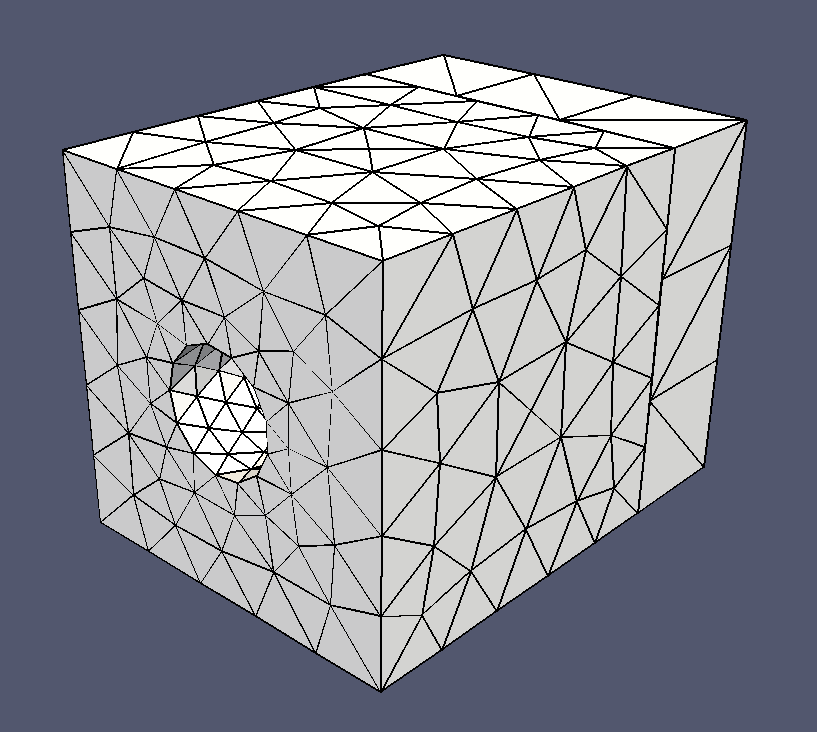
\includegraphics[width=0.5\textwidth]{images/ecartInversionGrid_manual.png}
  \caption{Example of an external Cartesian inversion grid created by Cubit}
  \label{basic_steps,sec:invgrid,sub:ecart,fig:grid}
\end{figure}

The nodes and cell files, e.g.\ produced by \lcode{Cubit}, are referred to in a parameter file, a template 
of which is file \lcode{template/ecartInversionGrid_parfile_template}. In the following, the particular 
parameters are explained. An example inversion grid of this type is displayed in 
figure~\myref{basic_steps,sec:invgrid,sub:ecart,fig:grid}.

%- - - - - - - - - - - - - - - - - - - - - - - - - - - - - 
\subsubsection{\lcode{ECART_INVGRID_USE_NODES_COMMON}}
Logical value to indicate whether to use one common nodes coordinates file for 
all cell types (only use parameter \lcode{ECART_INVGRID_FILE_NODES} below), or to use an individual 
nodes coordinates file for each cell type (use parameters files \lcode{ECART_INVGRID_FILE_NODES_TET4}, 
\lcode{ECART_INVGRID_FILE_NODES_HEX8}, \dots below).\\
When using module \lcode{cubit2ASKIecartInversionGrid} you should set:\\
\lcode{ECART_INVGRID_USE_NODES_COMMON = .True.}
%- - - - - - - - - - - - - - - - - - - - - - - - - - - - - 
\subsubsection{\lcode{ECART_INVGRID_FILE_NODES_COMMON}}
File name relative to \lcode{MAIN_PATH_INVERSION/ITERATION_STEP_PATH/} of nodes coordinates file to be commonly used
for definition of cells of all types in case of \lcode{ECART_INVGRID_USE_NODES_COMMON = .True.}\\
When using module \lcode{cubit2ASKIecartInversionGrid} you should set:\\
\lcode{ECART_INVGRID_FILE_NODES_COMMON = node_coordinates}
%- - - - - - - - - - - - - - - - - - - - - - - - - - - - - 
\subsubsection{\lcode{ECART_INVGRID_FILE_NODES_TET4}}
File name relative to \lcode{MAIN_PATH_INVERSION/ITERATION_STEP_PATH/} of nodes coordinates file to be used
for definition of tet4-type cells in case of \lcode{ECART_INVGRID_USE_NODES_COMMON = .False.}\\
%- - - - - - - - - - - - - - - - - - - - - - - - - - - - - 
\subsubsection{\lcode{ECART_INVGRID_FILE_NODES_HEX8}}
File name relative to \lcode{MAIN_PATH_INVERSION/ITERATION_STEP_PATH/} of nodes coordinates file to be used
for definition of hex8-type cells in case of \lcode{ECART_INVGRID_USE_NODES_COMMON = .False.}\\
%- - - - - - - - - - - - - - - - - - - - - - - - - - - - - 
\subsubsection{\lcode{ECART_INVGRID_FILE_CELLS_TET4}}
File name relative to \lcode{MAIN_PATH_INVERSION/ITERATION_STEP_PATH/} of cell connectivity file for 
definition of tet4-type cells.\\
When using module \lcode{cubit2ASKIecartInversionGrid} you should set:\\
\lcode{ECART_INVGRID_FILE_CELLS_TET4 = cell_connectivity_tet4}
%- - - - - - - - - - - - - - - - - - - - - - - - - - - - - 
\subsubsection{\lcode{ECART_INVGRID_FILE_CELLS_HEX8}}
File name relative to \lcode{MAIN_PATH_INVERSION/ITERATION_STEP_PATH/} of cell connectivity file for 
definition of hex8-type cells.\\
When using module \lcode{cubit2ASKIecartInversionGrid} you should set:\\
\lcode{ECART_INVGRID_FILE_CELLS_HEX8 = cell_connectivity_hex8}
%- - - - - - - - - - - - - - - - - - - - - - - - - - - - - 
\subsubsection{\lcode{ECART_INVGRID_FILE_NEIGHBOURS}}
File name relative to \lcode{MAIN_PATH_INVERSION/ITERATION_STEP_PATH/} of cell neighbours file. If not
present, this file will be created when first using the inversion grid. If present, its content defines 
the neighbour structure of the inversion grid cells. If, however, the inversion grid
is to be recreated (e.g.\ when calling \lcode{initBasics -recr}, see section~\myref{basic_steps,sec:initBasics}),
this file is recreated.
%- - - - - - - - - - - - - - - - - - - - - - - - - - - - - 
\subsubsection{\lcode{ECART_INVGRID_FILE_NEIGHBOURS_IS_BINARY}}
Logical value to indicate whether \lcode{ECART_INVGRID_FILE_NEIGHBOURS} should be binary or not.
%- - - - - - - - - - - - - - - - - - - - - - - - - - - - - 
\subsubsection{\lcode{SCALE_VTK_COORDS,VTK_COORDS_SCALING_FACTOR}}
Scale vtk geometry coordinates by factor \lcode{VTK_COORDS_SCALING_FACTOR} (real number), if 
\lcode{SCALE_VTK_COORDS = .true.}. This may be helpful if coordinate values (e.g.\ in meters) 
get so large that they cause problems when plotting in paraview.\\
Example:\\
\lcode{SCALE_VTK_COORDS = .false.}\\
\lcode{VTK_COORDS_SCALING_FACTOR = 1.0}
%
%----------------------------------------------------------
\subsection{\lcodetitle{specfem3dInversionGrid}} \label{basic_steps,sec:invgrid,sub:specfem3d}
%----------------------------------------------------------
%
An inversion grid of type \lcode{specfem3dInversionGrid} is method dependent and is to be used with 
\lcode{METHOD = SPECFEM3D} only. Whole spectral elements are used as inversion grid cells and all 
GLL points inside such an element as the wavefield points. All information regarding the element 
geometry, including information on neighbour cells and the values of the jacobian for every wavefield 
point contained in an element are read from files which are produced by \lcode{SPECFEM3D} methods.

Every type of integration weights is supported by this type of inversion grid, including weights of type 
\lcode{6} (external integration weights).

Please refer to the documentation of your \lcode{SPECFEM3D} forward method (\myref{basic_steps,sec:forward_problem})
on how to define an inversion grid of type \lcode{specfem3dInversionGrid}.
%
%++++++++++++++++++++++++++++++++++++++++++++++++++++++++++
\section{Define a Starting Model} \label{basic_steps,sec:start_model}
%++++++++++++++++++++++++++++++++++++++++++++++++++++++++++
%
There are two possibilities to define an earth model for the forward wave propagation in your first iteration:

On the one hand you may use any (standard) earth model provided by the forward method you are using, if appropriate.

If this is not possible, or the models provided do not meet your needs, you may use binary 
\lcode{createStartmodelKim} along with the inversion grid of your first iteration (which you should 
have already defined) to produce an inverted model file containing some simple model on this inversion grid. 
\lcode{createStartmodelKim -h} will print a help message how to use the program. Afterwards you may 
export the produced model file to your forward method as explained in section~\myref{basic_steps,sec:export_kim}.
%
%++++++++++++++++++++++++++++++++++++++++++++++++++++++++++
\section{Export Inverted Model} \label{basic_steps,sec:export_kim}
%++++++++++++++++++++++++++++++++++++++++++++++++++++++++++
%
The binary program \lcode{exportKim} exports an inverted model file (``kim'' stands for ``K''ernel 
``I''nverted ``M''odel) along with the respective inversion grid specifications to a text file, 
which may be used to communicate such a model to a forward method or postprocess the model values in any way. 
\lcode{exportKim -h} will print a help message how to use it. Template files of starting model descriptions
may be found in \lcode{template/}.
%
%++++++++++++++++++++++++++++++++++++++++++++++++++++++++++
\section{Solving the Forward Problem} \label{basic_steps,sec:forward_problem}
%++++++++++++++++++++++++++++++++++++++++++++++++++++++++++
%
In the following, all wave propagation codes which are supported by \ASKI are listed.
Refer to the given documentation on any details regarding the interaction of the forward codes with \ASKI.
\subsection*{\lcode{Gemini II}}
\lcode{Gemini II} is not yet fully supported in this release version. For some test cases, waveform kernels were
successfully computed using \lcode{Gemini II} in Cartesian as well as spherical setting. We hope to provide the 
\lcode{Gemini II} interface for \ASKI soon.
\subsection*{\lcode{SPECFEM3D_Cartesian}}
The Cartesian spectral element code \lcode{SPECFEM3D_Cartesian} is supported by \ASKI, 
cf.~\cite{Specfem3D_Cartesian_for_ASKI}
\subsection*{\lcode{SPECFEM3D_GLOBE}}
The global spectral element code \lcode{SPECFEM3D_GLOBE} is not yet fully supported in this release version. 
For some test cases, waveform kernels were successfully computed using \lcode{SPECFEM3D_GLOBE}. We hope to 
provide the \lcode{SPECFEM3D_GLOBE} interface for \ASKI soon.
%
%++++++++++++++++++++++++++++++++++++++++++++++++++++++++++
\section{Choose Integration Weights} \label{basic_steps,sec:intw}
%++++++++++++++++++++++++++++++++++++++++++++++++++++++++++
%
In order to numerically integrate the sensitivity kernels, which are computed on the wavefield points, 
over the inversion grid cells by a weightet summation of values, there are different 
types of integration weights provided, following different rules of integration.

The integer values of the type have the following meaning:
\begin{itemize}
  \item[] \lcode{0} $\rightarrow$ all weights are the same, \lcode{weight = 1/number_of_points_in_box}, 
    i.e.\ no integration(!), just building the average sensitivity value (e.g.\ convenient for comparison of 
    sensitivities computed with different methods on different forward grids)
  \item[] \lcode{1} $\rightarrow$ Scattered Data Integration, as in \cite{Levin99}, polynomial degree 1
  \item[] \lcode{2} $\rightarrow$ Scattered Data Integration, as in \cite{Levin99}, polynomial degree 2, 
    i.e.\ approximation order 3 (?)
  \item[] \lcode{3} $\rightarrow$ Scattered Data Integration, as in \cite{Levin99}, polynomial degree 3, 
    i.e.\ approximation order 4 (?)
  \item[] \lcode{4} $\rightarrow$ for each cell, compute the highest possible order of Scattered Data Iintegration
    integration after \cite{Levin99} (trying types 3,2,1 (in that order) until computation was successful)
  \item[] \lcode{5} $\rightarrow$ average of function values, multiplied with volume of box (i.e.\ $\sim$ linear integration)
  \item[] \lcode{6} $\rightarrow$ external integration weights, to be used along with a suitable inversion grid 
    (e.g.\ of type \lcode{specfem3dInversionGrid}, see section~\myref{basic_steps,sec:invgrid,sub:specfem3d})
\end{itemize}

A detailed description of some of the integration weights, especially the weights after \cite{Levin99} can be found in 
section~\myref{programs_scripts,sec:fmod_intw}.
%
%++++++++++++++++++++++++++++++++++++++++++++++++++++++++++
\section{Create a Data and Model Space} \label{basic_steps,sec:dmspace}
%++++++++++++++++++++++++++++++++++++++++++++++++++++++++++
%
In order to choose a set of data samples which to invert and a set of model parameters which to invert for, 
you need to define a data space and a model space. Essentially, if you have $m$ data samples, the space in which 
the data live is just \R m (analogously, for $n$ model parameters, the model lives in \R n ). You only need to define which
data sample (model parameter) refers to which dimension (i.e.\ entry in vector) of the data space (model space).\\
The $m\times n$ sensitivity kernel matrix will then connect a vector of model updates from model space in \R n 
to your specific data vector from \R m.

In the following, we describe how data samples and model parameters are defined in this software package and how you can 
choose specific subsets to be used. 
%----------------------------------------------------------
\subsection{Definition of Data Samples}
%----------------------------------------------------------
As the sensitivities are calculated in frequency domain, the data live in frequency domain, too.\\
A data sample is uniquely characterized by a seismic \emph{source}, a \emph{component} 
of a seismic \emph{receiver}, and a \emph{frequency}, as well as if it is \emph{real} or \emph{imaginary} part 
of the complex spectral values. Refer to \myref{basic_steps,sec:data_general} for details on data in \ASKI.
%----------------------------------------------------------
\subsection{Definition of Model Parameters} \label{basic_steps,sec:dmspace,sub:mparam}
%----------------------------------------------------------
A model parameter is uniquely  characterized by a parameter name (mus be a valid parameter name of the model
parametrization as defined by \lcode{MODEL_PARAMETRIZATION} \myref{files,sec:main_parfile,itm:mod_pmtrz}) 
and an inversion grid cell index in valid range.
%----------------------------------------------------------
\subsection{Choosing a Set of Data Samples and Model Parameters}
%----------------------------------------------------------
Create a text file as described in section \myref{files,sec:dmspace}.
%
%++++++++++++++++++++++++++++++++++++++++++++++++++++++++++
\section{Initiate Basic Requirements} \label{basic_steps,sec:initBasics}
%++++++++++++++++++++++++++++++++++++++++++++++++++++++++++
%
Run binary \lcode{initBasics}, \lcode{initBasics -h} will print a help message how to use it.

It first checks if all parameters needed are present in the parameter files and then creates all
basic requirements for \ASKI operations:\\
It reads in required files like event list and station list files, the wavefield points and the 
kernel reference model. \\
Furthermore, it creates the inversion grid (possibly storing some inversion grid files, dependent 
on the type of grid), localizes the wavefield points inside it and computes 
the integration weights, which are written to file. Once those files exist, \lcode{initBasics} 
and all other programs will always read the integration weights (and possibly (part of) the inversion grid) 
from file, \emph{regardless} of what the parameter files say! So if at some you point want to use 
different integration weights or a different inversion grid, you will have to either delete the respective 
file(s) and rerun \lcode{initBasics}, or run \lcode{initBasics -recr} in order
to recreate them. 

Also a lot of \lcode{.vtk} files with statistics are produced having base filename \lcode{FILEBASE_BASIC_STATS} as 
defined in the parameter file of the current iteration step. Those files mainly regard the inversion grid, 
the wavefield points and the integration weights, whereby the respective filenames are extended (by something 
with ``.vtk''). It is \emph{highly recommended} to call \lcode{initBasics -recr} in order to assure that all
those \lcode{.vtk} files are produced and to actually have a look at them before continuing any \ASKI operation!
%
%++++++++++++++++++++++++++++++++++++++++++++++++++++++++++
\section{Compute Standard Sensitivity Kernels} \label{basic_steps,sec:compute_kernels}
%++++++++++++++++++++++++++++++++++++++++++++++++++++++++++
%
The kernels are computed by combining green tensor and forward wavefield for a given path, and
by integration over all inverison grid cells. I.e.\ there is one sensitivity kernel file for a
specific path. This file contains sensitivity values of the three Cartesian receiver components 
\lcode{CX}, \lcode{CY}, \lcode{CZ} for all model parameters of your model parametrization, with 
the values living on the inverison grid cells.

Use binary \lcode{computeKernels}. \lcode{computeKernels -h} will print a help message how to use it.
It makes sense, to only compute kernel files for those paths that you are going to use (defined by
your data model space file).

You can define the set of paths for which sensitivities should be computed in two ways:
\begin{itemize}
\item[way 1] compute a kernel for only one path, defined by eventID and station name using options \lcode{-evid} 
and \lcode{-stname}
\item[way 2] input a data and model space file (as defined by \myref{basic_steps,sec:dmspace}) by option 
\lcode{-dmspace}, defining all paths for which kernels should be computed; optionally define range of path index
by \lcode{-ipath1}, \lcode{-ipath2}
\end{itemize}
%
%++++++++++++++++++++++++++++++++++++++++++++++++++++++++++
\section{Transform to Time-Domain Sensitivity Kernels} \label{basic_steps,sec:compute_time_kernels}
%++++++++++++++++++++++++++++++++++++++++++++++++++++++++++
%
The time kernels are computed from the standard frequency-domain kernels (which were computed path-wise)
by applying an inverse Fourier transform. The transforation is done for specific data components
(e.g. \lcode{N}, \lcode{DOWN}, \lcode{CY}, ..), where first the spectra for the standard component 
\lcode{CX}, \lcode{CY}, \lcode{CZ} are rotated and afterwards the respective event filter and station component
filter are applied before the actual Fourier transform takes place.

Use binary \lcode{spec2timeKernels}. \lcode{spec2timeKernels -h} will print a help message how to use it.
It makes sense, to only compute kernel files for those paths that you are going to use (defined by
your data model space file).

You can define the set of paths for which the time-domain kernels should be computed in two ways:
\begin{itemize}
\item[way 1] transform a kernel for only one path, defined by eventID and station name using options \lcode{-evid} 
and \lcode{-stname}
\item[way 2] input a data and model space file (as defined by \myref{basic_steps,sec:dmspace}) by option 
\lcode{-dmspace}, defining all paths for which kernels should be transformed; optionally define range of path index
by \lcode{-ipath1}, \lcode{-ipath2}
\end{itemize}
%
%++++++++++++++++++++++++++++++++++++++++++++++++++++++++++
\section{Plot Standard Sensitivity Kernels} \label{basic_steps,sec:plot_kernels}
%++++++++++++++++++++++++++++++++++++++++++++++++++++++++++
%
One way to plot a specific sensitivity Kernel in frequency domain, i.e.\ the sensitivity spectra for a specific
path, is to procuce vtk files with binary \lcode{kernel2vtk}. \lcode{kernel2vtk -h} will print a help message 
how to use it.\\
Please note, that the output \lcode{.vtk} files (one for every frequency) might get large, dependent on the resolution 
of the inversion grid, since the geometry information of the inversion grid cells is contained in each \lcode{.vtk} file.
%
%++++++++++++++++++++++++++++++++++++++++++++++++++++++++++
\section{Plot Time Sensitivity Kernels} \label{basic_steps,sec:plot_time_kernels}
%++++++++++++++++++++++++++++++++++++++++++++++++++++++++++
%
One way to plot a specific sensitivity Kernel in time domain, is to procuce vtk files with binary \lcode{timeKernel2vtk}. 
\lcode{timeKernel2vtk -h} will print a help message how to use it.\\
Please note, that the output \lcode{.vtk} files (one for every time step) might get large, dependent on the resolution 
of the inversion grid, since the geometry information of the inversion grid cells is contained in each \lcode{.vtk} file.
%
%++++++++++++++++++++++++++++++++++++++++++++++++++++++++++
\section{Solve Kernel System} \label{basic_steps,sec:solve_kernel_system}
%++++++++++++++++++++++++++++++++++++++++++++++++++++++++++
%
Call binary \lcode{solveKernelSystem} to set up the kerne matrix, read in synthetic
and real data, add smoothing (if required). \lcode{solveKernelSystem -h} will print a help message how to use it.

%%% Local Variables:
%%% mode: latex
%%% TeX-master: "manual"
%%% End:

%
%-------------------------------
% APPENDIX CONTAINING CHAPTERS WITH MORE DETAILS
%\appendix
%
%-------------------------------
% APPENDIX CHAPTER file formats
\chapter{Files} %\label{files}
% -*-LaTex-*-

%-----------------------------------------------------------------------------
%   Copyright 2016 Florian Schumacher (Ruhr-Universitaet Bochum, Germany)
%
%   This file is part of the ASKI manual as a LaTeX document with main file
%   manual.tex
%
%   Permission is granted to copy, distribute and/or modify this document
%   under the terms of the GNU Free Documentation License, Version 1.3
%   or any later version published by the Free Software Foundation;
%   with no Invariant Sections, no Front-Cover Texts, and no Back-Cover Texts.
%   A copy of the license is included in the section entitled ``GNU
%   Free Documentation License''. 
%-----------------------------------------------------------------------------
%
This chapter collects documentation on file formats involved in \ASKI{}.
%
%++++++++++++++++++++++++++++++++++++++++++++++++++++++++++
\section{Parameter Files} \label{files,sec:parfiles}
%++++++++++++++++++++++++++++++++++++++++++++++++++++++++++
%
Parameter files are simple text files.

The following type of lines are ignored:
\begin{itemize}
\item comment lines, i.e.\ lines STARTING with an arbitrary number of blanks followed by a ``\#'' character
\item empty lines and lines containing blanks only
\item lines not containing any ``='' character
\end{itemize}

How to specify one parameter:
\begin{itemize}
\item valid lines have the form ``keyword = value'' (blanks leading or following ``keyword'', ``='', or ``value'' are ignored)
\item in a valid line, all characters in front of ``='' (without leading and appending blanks)
are interpreted as the keyword, allowing for blank characters within the keyword (e.g.\ for lines  
\mbox{``\hspace{5mm}key~word~=~value\hspace{3mm}''}, the string ``key~word'' is used as the keyword)
\item all characters behind ``='' (without leading and appending blanks) are interpreted as the value string from 
which the value is read, which in particular means that ``\#'' comments at the end of a line (such as 
\mbox{``\hspace{3mm}keyword = value\hspace{2mm}\# comment\hspace{3mm}''}) are \emph{not} allowed!
\end{itemize}
By convention, specify \emph{paths} (i.e.\ directory names, which will be concatenated with a filename of 
a file in that directory) always ending on ``/'' and specify \emph{filenames} always \emph{without} leading ``/''.
%
%----------------------------------------------------------
\subsection{Main Parameter File} \label{files,sec:main_parfile}
%----------------------------------------------------------
%
Here, shortly all keywords required in the main parameter file for your specific program operation, are described.
%- - - - - - - - - - - - - - - - - - - - - - - - - - - - - 
\subsubsection{\lcode{FORWARD_METHOD}} \label{files,sec:main_parfile,itm:forward_method}
\begin{itemize}
\item[] \lcode{GEMINI}
\item[] \lcode{SPECFEM3D} $\rightarrow$ \lcode{SPECFEM3D_Cartesian} and \lcode{SPECFEM3D_GLOBE}
\item[] \lcode{NEXD} 
\end{itemize}
For details on the methods and references to their documentation, refer to section~\ref{basic_steps,sec:forward_problem}
%- - - - - - - - - - - - - - - - - - - - - - - - - - - - -
\subsubsection{\lcode{MODEL_PARAMETRIZATION}} \label{files,sec:main_parfile,itm:mod_pmtrz}
\begin{itemize}
\item[] \lcode{isoLameSI} $\rightarrow$ isotropic Lam\'e parameters and density in SI units: 
    $\rho$ (\lcode{rho}) [kg/m\textsuperscript{3}], $\lambda$ (\lcode{lambda}) [Pa], $\mu$ (\lcode{mu})  [Pa]
\item[] \lcode{isoVelocitySI} $\rightarrow$ isotropic seismic velocities and density in SI units:
    $\rho$ (\lcode{rho}) [kg/m\textsuperscript{3}], $v_p$ (\lcode{vp}) [m/s], $v_s$ (\lcode{vs}) [m/s]
\item[] \lcode{isoVelocity1000} $\rightarrow$ isotropic seismic velocities and density in  
  units involving a factor of 1000: $\rho$ (\lcode{rho}) [g/cm\textsuperscript{3}], $v_p$ (\lcode{vp}) [km/s], 
  $v_s$ (\lcode{vs}) [km/s]
\end{itemize}
Nothing other parameterization supported yet.
%- - - - - - - - - - - - - - - - - - - - - - - - - - - - - 
\subsubsection{\lcode{PARAMETER_CORRELATION_MODE}} \label{files,sec:main_parfile,itm:par_cor_mode}
Any model parameters can be correlated to others which are not inverted for. So far supported correlation modes:
\begin{itemize}
\item[] \lcode{NONE} $\rightarrow$ no parameter correlation will be done whatsoever
\item[] \lcode{CORRELATE_KERNELS} $\rightarrow$ will add correlated kernel values of other parameters to the kernels
  of those parameters which are inverted for (experimental feature, not yet tested in practice).
\end{itemize}
%- - - - - - - - - - - - - - - - - - - - - - - - - - - - -
\subsubsection{\lcode{PARAMETER_CORRELATION_FILE}} \label{files,sec:main_parfile,itm:par_cor_file}
File (relative to \lcode{MAIN_PATH_INVERSION}) containing the definition of the correlation and the correlation coefficients. 
The given filename is ignored in case of \lcode{PARAMETER_CORRELATION_MODE = NONE}.
%- - - - - - - - - - - - - - - - - - - - - - - - - - - - -
\subsubsection{\lcode{MAIN_PATH_INVERSION}} \label{files,sec:main_parfile,itm:main_path}
All subpaths for filenames are considered relative to this main path. This
directory is thought to contain all your relevant output and (temporary) data.\\
Example: \lcode{MAIN_PATH_INVERSION = /data/inversions/Aegean1/}
%- - - - - - - - - - - - - - - - - - - - - - - - - - - - -
\subsubsection{\lcode{CURRENT_ITERATION_STEP}} \label{files,sec:main_parfile,itm:cur_iter_step}
Example: \lcode{CURRENT_ITERATION_STEP = 3}
%- - - - - - - - - - - - - - - - - - - - - - - - - - - - - 
\subsubsection{\lcode{ITERATION_STEP_PATH}} \label{files,sec:main_parfile,itm:iter_path}
Relative to main path, defining name of subdirectory of \lcode{MAIN_PATH_INVERSION} which contains 
all relevant (meta)data of an inversion step. A three-digit integer (= \lcode{CURRENT_ITERATION_STEP}) 
and ``/'' will be appended to \lcode{ITERATION_STEP_PATH} (i.e.\ ``001/'', ``002/'', \dots) defining the 
first, second \dots iteration step directory.\\
Example (default): \lcode{ITERATION_STEP_PATH = iteration_step_}
%- - - - - - - - - - - - - - - - - - - - - - - - - - - - - 
\subsubsection{\lcode{PARFILE_ITERATION_STEP}} \label{files,sec:main_parfile,itm:iter_parfile}
File name of iteration step specific parameter file, relative to \lcode{MAIN_PATH_INVERSION/ITERATION_STEP_PATH}
Example: \lcode{PARFILE_ITERATION_STEP = iter_parfile}
%- - - - - - - - - - - - - - - - - - - - - - - - - - - - - 
\subsubsection{\lcode{PATH_MEASURED_DATA,APPLY_EVENT_FILTER,PATH_EVENT_FILTER,APPLY_STATION_FILTER,PATH_STATION_FILTER}} 
\label{files,sec:main_parfile,itm:path_mdata_filters}
Paths and flags related to the measured data. The paths are \emph{absolute}, i.e.\ can be everywhere, 
e.g.\ close to where you 
have stored/processed your (time domain) data, or in directory \lcode{MAIN_PATH_INVERSION}, etc.\ \dots

If you do not wish to use any filtering per events, you can switch to\\
\lcode{APPLY_EVENT_FILTER = .false.},\\
if you do not wish to use any fitering per stations, you can switch to\\
\lcode{APPLY_STATION_FILTER = .false.}.\\
In these cases, the respective filter files are not expected to exist and the respective filter paths are
ignored.

The naming convention of the files in the respective directories is:\\
\lcode{FILE_MEASURED_DATA}: \lcode{data_EVENTID_STATIONNAME_COMP},\\
\lcode{FILE_EVENT_FILTER}: \lcode{filter_EVENTID},\\
\lcode{FILE_STATION_FILTER}: \lcode{filter_STATIONNAME_COMP}, \\
where station filters are dependet on component and \lcode{STATIONNAME} and \lcode{EVENTID} are 
defined in \lcode{FILE_STATION_LIST} and \lcode{FILE_EVENT_LIST} file, and \lcode{COMP} 
is a valid component (for valid components see \ref{basic_steps,sec:data_general})\\
Example: \\
\lcode{PATH_MEASURED_DATA = /mydata/your_name_of_inversion/ASKI_data/}\\
\lcode{PATH_EVENT_FILTER = /mydata/your_name_of_inversion/ASKI_event_filter/}\\
\lcode{PATH_STATION_FILTER = /mydata/your_name_of_inversion/ASKI_station_filter/}\\

%- - - - - - - - - - - - - - - - - - - - - - - - - - - - - 
\subsubsection{\lcode{FILE_EVENT_LIST}} \label{files,sec:main_parfile,itm:file_event_list}
Absolute filename where \ASKI{} finds a text file defining a set of events in the required format 
(\ref{files,sec:event_list})\\
Example: \lcode{FILE_EVENT_LIST = /mydata/your_name_of_inversion/ASKI_events}
%- - - - - - - - - - - - - - - - - - - - - - - - - - - - - 
\subsubsection{\lcode{FILE_STATION_LIST}} \label{files,sec:main_parfile,itm:file_station_list}
Absolute filename where \ASKI{} finds a text file defining a set of stations in the required format 
(\ref{files,sec:station_list})\\
Example: \lcode{FILE_STATION_LIST = /mydata/your_name_of_inversion/ASKI_stations}
%- - - - - - - - - - - - - - - - - - - - - - - - - - - - - 
\subsubsection{\lcode{MEASURED_DATA_FREQUENCY_STEP,MEASURED_DATA_NUMBER_OF_FREQ,MEASURED_DATA_INDEX_OF_FREQ}} 
\label{files,sec:main_parfile,itm:mdata_freq}
Discretized frequency window of measured data (same expected in event\_filter/station\_filter!) given by a frequency 
step \lcode{FREQUENCY_STEP} [Hz] and a vector of frequency indices \lcode{INDEX_OF_FREQ}
(of length \lcode{NUMBER_OF_FREQ}), where for specific frequency index $i$ the corresponding frequency $f_i$ [Hz] 
computes to $f_i = i \cdot$ \lcode{FREQUENCY_STEP}\\
Example:\\
\lcode{MEASURED_FREQUENCY_STEP = 10.}\\
\lcode{MEASURED_NUMBER_OF_FREQ = 5}\\
\lcode{MEASURED_INDEX_OF_FREQ = 2 3 5 7 10}\\
which corresponds to the 5 frequencies $20,30,50,70,100$ Hz
%- - - - - - - - - - - - - - - - - - - - - - - - - - - - - 
\subsubsection{\lcode{UNIT_FACTOR_MEASURED_DATA}} 
Indicate the unit factor of the measured data. The definition of the factor is:\\
Multiplication of the measured data (displacement) with this factor gives values in the SI unit of meters [m].\\
Example: If you use seismic time-domain data for \ASKI{} in the unit of nano meters [nm], then \lcode{UNIT_FACTOR_MEASURED_DATA}
must be set to \lcode{1.0e-9} , because the data values in nano meters [nm] must be divided by $1.0\cdot 10^9$ in order to get meters [m].
If you use seismic displacement data in the SI unit of meters, then \lcode{UNIT_FACTOR_MEASURED_DATA} must be set to \lcode{1.0}.
%- - - - - - - - - - - - - - - - - - - - - - - - - - - - - 
\subsubsection{\lcode{DEFAULT_VTK_FILE_FORMAT}} 
Either \lcode{BINARY} or \lcode{ASCII} defining the default type of \lcode{vtk} files 
which will be produced in the course of running the programs.
%
%----------------------------------------------------------
\subsection{Parameter File for Specific Iteration Step} \label{files,sec:iter_parfile}
%----------------------------------------------------------
%
Here, shortly all keywords required in a parameter file for a specific iteration step, i.e.\ \\
\lcode{MAIN_PATH_INVERSION/ITERATION_STEP_PATH/PARFILE_ITERATION_STEP} , are described.

These parameter files are created automatically by script \lcode{py/create_ASKI_dir.py}. 
Alternatively, you can look at the template file \lcode{template/iter_parfile_template}.
%- - - - - - - - - - - - - - - - - - - - - - - - - - - - - 
\subsubsection{\lcode{USE_PATH_SPECIFIC_MODELS}}
Set the flag to \lcode{.true.} if you intend to use the \ASKI{} functionality of path specific kernel 
reference models (usually only for the very first iteration and a 1D method, as described in 
section~\myref{basic_steps,sec:path_specific}). For a regular iteration, i.e.\ using one 
global kernel reference model (for all paths, i.e.\ kernels) set this flag to \lcode{.false.}.
%- - - - - - - - - - - - - - - - - - - - - - - - - - - - - 
\subsubsection{\lcode{ITERATION_STEP_NUMBER_OF_FREQ, ITERATION_STEP_INDEX_OF_FREQ}} \label{files,sec:iter_parfile,itm:iter_freq}
Frequency discretization of this iteration step, must be a subset of global frequency discretization 
for this inversion defined as defined by \ref{files,sec:main_parfile,itm:mdata_freq}. \\
\lcode{ITERATION_STEP_NUMBER_OF_FREQ} must be smaller or equal to \lcode{MEASURED_DATA_NUMBER_OF_FREQ} and vector \\
\lcode{ITERATION_STEP_INDEX_OF_FREQ} (of length \lcode{ITERATION_STEP_NUMBER_OF_FREQ})
must only contain indices contained in \lcode{MEASURED_DATA_INDEX_OF_FREQ}.\\
All indices here are assumed in accordance with the global frequency step \lcode{MEASURED_DATA_FREQUENCY_STEP}.
%- - - - - - - - - - - - - - - - - - - - - - - - - - - - - 
\subsubsection{\lcode{TYPE_INVERSION_GRID, PARFILE_INVERSION_GRID}} \label{files,sec:iter_parfile,itm:invgrid}
Type of inversion grid (as supported, cf.\ \ref{basic_steps,sec:invgrid}) and corresponding
filename of parameter file defining this inversion grid, relative to \\
\lcode{MAIN_PATH_INVERSION/ITERATION_STEP_PATH/}
%- - - - - - - - - - - - - - - - - - - - - - - - - - - - - 
\subsubsection{\lcode{TYPE_INTEGRATION_WEIGHTS}}
Type of integration weights (integer number), cf.\ \ref{basic_steps,sec:intw} for supported values.
%- - - - - - - - - - - - - - - - - - - - - - - - - - - - - 
\subsubsection{\lcode{FILE_INTEGRATION_WEIGHTS}} 
Filename of the integration weights file, which will be created and used, relative to 
\lcode{MAIN_PATH_INVERSION}. 
%- - - - - - - - - - - - - - - - - - - - - - - - - - - - -
\subsubsection{\lcode{FILE_WAVEFIELD_POINTS}} 
Filename of the wavefield points file, relative to \lcode{MAIN_PATH_INVERSION}, which
is in general created by the method you are using. Just refer here to this file. 
%- - - - - - - - - - - - - - - - - - - - - - - - - - - - -
\subsubsection{\lcode{FILE_KERNEL_REFERENCE_MODEL}} \label{files,sec:iter_parfile,itm:model}
Dependent on the method you are using, these filenames may be handled individually. Please refer to the respective 
documentation of the methods for recommendations how to use these parameters, or which naming to choose.
%- - - - - - - - - - - - - - - - - - - - - - - - - - - - - 
\subsubsection{\lcode{FILEBASE_BASIC_STATS}}
Base filename of vtk stats output files (related to inversion grid, wavefield points, integration weights,
events, stations), relative to \lcode{MAIN_PATH_INVERSION/ITERATION_STEP_PATH}. 
%- - - - - - - - - - - - - - - - - - - - - - - - - - - - - 
\subsubsection{\lcode{PATH_OUTPUT_FILES}}
Folder relative to which some sensitivity analysis and inversion programs may write their output (relatively small output
like models, coefficients etc., NO wavefields/kernels etc.!), relative to 
\lcode{MAIN_PATH_INVERSION/ITERATION_STEP_PATH}.  Make sure the path ends on ``/".
%- - - - - - - - - - - - - - - - - - - - - - - - - - - - -
\subsubsection{\lcode{PATH_KERNEL_DISPLACEMENTS}} 
Subdirectory of current iteration step path
\lcode{MAIN_PATH_INVERSION/ITERATION_STEP_PATH} which contains the 
kernel displacement files. Make sure the path ends on ``/".
%- - - - - - - - - - - - - - - - - - - - - - - - - - - - -
\subsubsection{\lcode{PATH_KERNEL_GREEN_TENSORS}} 
Subdirectory of current iteration step path
\lcode{MAIN_PATH_INVERSION/ITERATION_STEP_PATH} which contains the 
kernel green tensor files. Make sure the path ends on ``/".
%- - - - - - - - - - - - - - - - - - - - - - - - - - - - -
\subsubsection{\lcode{PATH_SENSITIVITY_KERNELS}} 
Subdirectory of current iteration step path
\lcode{MAIN_PATH_INVERSION/ITERATION_STEP_PATH} which contains the 
velocity kernel files. Make sure the path ends on ``/".
%- - - - - - - - - - - - - - - - - - - - - - - - - - - - -
\subsubsection{\lcode{PATH_SYNTHETIC_DATA}} 
Subdirectory of current iteration step path
\lcode{MAIN_PATH_INVERSION/ITERATION_STEP_PATH} which contains the 
files with synthetic data. Make sure the path ends on ``/".
%- - - - - - - - - - - - - - - - - - - - - - - - - - - - -
\subsubsection{\lcode{PATH_KERNEL_REFERENCE_MODELS}} 
This path and any contained files are only relevant for \lcode{USE_PATH_SPECIFIC_MODELS = .true.}!
Subdirectory of current iteration step path
\lcode{MAIN_PATH_INVERSION/ITERATION_STEP_PATH} in which path-specific kernel reference models are expected.
The reference model files are assumed to have names like \lcode{krm_EVENTID_STATIONNAME}.
Make sure the path ends on ``/".

%
%++++++++++++++++++++++++++++++++++++++++++++++++++++++++++
\section{Event List File} \label{files,sec:event_list}
%++++++++++++++++++++++++++++++++++++++++++++++++++++++++++
%
Please find the template event list file \lcode{template/file_event_list_template}.

\begin{itemize}
\item first line contains single character ``C'' or ``S'', defining the coordinate system (``C''artesian or ``S''pherical)
  with respect to which the given event coordinates lat,lon are interpreted
\item each following non-empty line of the file is interpreted as a definition of one event and must 
  contain the following space-separated values:
  \begin{itemize}
  \item[eventid]  13 character name, (e.g. \lcode{2006.10.2977} or \lcode{061113_141238}) 
    should \emph{not} contain whitespace!
  \item[origintime]  characters of form \lcode{yyyymmdd_hhmmss_nnnnnnnnn} or \lcode{yyyymmdd_hhmmss}
    (i.e.\ with or without nano-seconds), e.g. \lcode{20130320_170012} or 
    \lcode{20130320_170002_718000000}
  \item[lat] latitude in degrees, \lcode{-90 <= lat <= 90} (``S'') or first coordinate in 
    wavefield points / inversion grid - frame (``C'') $\rightarrow$  read the section on inversion grid definitions 
    (\ref{basic_steps,sec:invgrid})
  \item[lon] longitude in degrees, \lcode{0 <= lon <= 360} (``S'') or second  coordinate in 
    wavefield points / inversion grid -frame (``C'') (read \ref{basic_steps,sec:invgrid})
  \item[depth] source depth in km (``S''), or third coordinate in wavefield points / inversion grid -frame (``C'') 
    (read \ref{basic_steps,sec:invgrid})
  \item[mag] factor on source mechanism
  \item[typ] source type:  0 = force, 1 = moment tensor, -1: not specified
  \item[mom/frce] either 3 values (force vector) or 6 values (moment tensor)
  \end{itemize}
\end{itemize}
%
%++++++++++++++++++++++++++++++++++++++++++++++++++++++++++
\section{Station List File} \label{files,sec:station_list}
%++++++++++++++++++++++++++++++++++++++++++++++++++++++++++
%
Please find the template station list file \lcode{template/file_station_list_template}.

\begin{itemize}
\item first line contains single character ``C'' or ``S'', defining the coordinate system (``C''artesian or ``S''pherical)
  with respect to which the given event coordinates lat,lon are interpreted
\item each following non-empty line of the file is interpreted as a definition of one station and must 
  contain the following space-separated values:
  \begin{itemize}
  \item[station\_name] 5 character name, which should \emph{neither} contain whitespace \emph{nor} underscors ``\_''!
  \item[network\_code] 6 character network code
  \item[lat] latitude in degrees, \lcode{-90 <= lat <= 90} (``S'') or first coordinate in 
    wavefield points / inversion grid - frame (``C'') $\rightarrow$  read the manual on inversion grid definitions 
    (\ref{basic_steps,sec:invgrid})
  \item[lon] longitude in degrees, \lcode{0 <= lon <= 360} (``S'') or second  coordinate in 
    wavefield points / inversion grid -frame (``C'') (read \ref{basic_steps,sec:invgrid})
  \item[elevation] altitude of station (``S''), or third coordinate in wavefield points / inversion grid -frame (``C'') (read \ref{basic_steps,sec:invgrid})
  \end{itemize}
\end{itemize}
%
%++++++++++++++++++++++++++++++++++++++++++++++++++++++++++
\section{Measured Data Files} \label{files,sec:measured_data}
%++++++++++++++++++++++++++++++++++++++++++++++++++++++++++
%
All measured data files are expected to be located in the directory \lcode{PATH_MEASURED_DATA} as defined
in the main parameter file.

One measured data file contains all data values for one specific station component and a specific event.
Its filename is by convention \lcode{data_EVENTID_STATIONNAME_COMP}

The files are text files containing $1$ column of \lcode{MEASURED_DATA_NUMBER_OF_FREQ} complex numbers, 
which can be understood by \lcode{FORTRAN} \lcode{read} command, i.e.\ of form \lcode{( real_part , imag_part )} .

Line \lcode{i} contains the measured data value for the \lcode{i}\textsuperscript{th} frequency, as defined by vector
of indices \lcode{MEASURED_DATA_INDEX_OF_FREQ} and frequency step \lcode{MEASURED_DATA_FREQUENCY_STEP}. \\
In particular, this means that \emph{all} measured data files must contain the \emph{same} frequency discretization, given
by parameters \lcode{MEASURED_DATA_INDEX_OF_FREQ}, \lcode{MEASURED_DATA_FREQUENCY_STEP} of the main 
parameter file.
%
%++++++++++++++++++++++++++++++++++++++++++++++++++++++++++
\section{Event (Station) Filter Files} \label{files,sec:filters}
%++++++++++++++++++++++++++++++++++++++++++++++++++++++++++
%
All event (or station) filter files are expected to be located in the directory \lcode{PATH_EVENT_FILTER} 
(or \lcode{PATH_STATION_FILTER}), respectively. Both paths savely be set to the same directory.

A filter file contains all spectral filter values associated with a specific event (or station component). 
The file names are by convention \lcode{filter_EVENTID} (or \lcode{filter_STATIONNAME_COMP}), respectively.

In the same way as measured data files, the filter files are text files containing $1$ column of 
\lcode{MEASURED_DATA_NUMBER_OF_FREQ} complex numbers, 
which can be understood by \lcode{FORTRAN} \lcode{read} command, i.e.\ of form \lcode{( real_part , imag_part )} .

Line \lcode{i} contains the filter value for the \lcode{i}\textsuperscript{th} frequency, as defined by vector
of indices \lcode{MEASURED_DATA_INDEX_OF_FREQ} and frequency step \lcode{MEASURED_DATA_FREQUENCY_STEP}. \\
In particular, this means that \emph{all} filter files must contain the \emph{same} frequency discretization, given
by parameters \lcode{MEASURED_DATA_INDEX_OF_FREQ}, \lcode{MEASURED_DATA_FREQUENCY_STEP} of the main 
parameter file.
%
%++++++++++++++++++++++++++++++++++++++++++++++++++++++++++
\section{Synthetic Data Files} \label{files,sec:synth_data} 
%++++++++++++++++++++++++++++++++++++++++++++++++++++++++++
%
All synthetic data files are expected to be in the directory \lcode{PATH_SYNTHETIC_DATA} as defined 
in the parameter file of the current iteration step.

One synthetic data file contains the complete synthetic data values for one specific combination of
event, station and station component. Its filename is by convention \lcode{synthetics_EVENTID_STATIONNAME_COMP}

The files are text files containing $1$ column of \lcode{ITERATION_STEP_NUMBER_OF_FREQ}  
complex numbers, which can be understood by \lcode{FORTRAN} \lcode{read} command, i.e.\ of form \lcode{( real_part , imag_part )} .

Line \lcode{i} contains the synthetic data value for the \lcode{i}\textsuperscript{th} frequency, as defined by vector
of indices \lcode{ITERATION_STEP_INDEX_OF_FREQ} and frequency step \lcode{MEASURED_DATA_FREQUENCY_STEP}.
%
%++++++++++++++++++++++++++++++++++++++++++++++++++++++++++
\section{Vtk Files} \label{files,sec:vtk_files}
%++++++++++++++++++++++++++++++++++++++++++++++++++++++++++
%
For visualization of basic objects of the inversion, such as the inversion grid, 
the wavefield points, the integration weights etc., as well as some inversion results
and models, we use the \lcode{vtk} file format. The files contain \emph{both}, geometry
information and data values on geometric objects. The format can be either \lcode{ASCII} or 
\lcode{BINARY}, controlled by flag \lcode{DEFAULT_VTK_FILE_FORMAT} in main parfile.\\
General information on this file format may be found under \url{www.vtk.org/VTK/img/file-formats.pdf}

\ASKI{} uses separate software modules for writing \lcode{vtk} based on wavefield points, or 
inversion grids or event-station path lines (or event, station coorrdinates). 
%
%++++++++++++++++++++++++++++++++++++++++++++++++++++++++++
\section{Data and Model Space File} \label{files,sec:dmspace}
%++++++++++++++++++++++++++++++++++++++++++++++++++++++++++
%
Files in which a data and model space is defined have the following form. \emph{It might be very instructive 
to also have a look at the provided example template files} \lcode{template/data_model_space_info_template_*} .

The blocks described in the subsections below should be put into a text file, one after another, in arbitrary order, 
i.e.\ it does not matter which block comes first (DATA SAMPLE or MODEL VALUES). It is
also supported to provide only one of the blocks, if the other one is not required for some application. 

\emph{There can be arbitrary commentary in front of a block, between blocks and after the blocks.} However, 
any line starting with \lcode{DATA SAMPLES} or \lcode{MODEL VALUES} is interpreted as the starting line
of the respective block. Inside the blocks, ther must not be unexpected lines!

%The header block must come first, then the data space block and model parameter block. The order of the latter two is arbitrary, both orders are allowed. %% IN CASE OF INTRODUCING SOME HEADER BLOCK IN THE FUTURE

%% %---------------------------------------------------------
%% \subsection{Header Block}
%% %---------------------------------------------------------
%% {\bf line 1}: currently ignored (file format version specification possible, header comment)

%% {\bf line 2}: must either contain \lcode{ASCII} or \lcode{BINARY}\\
%% At the moment, this file must be a formatted text file (nothing else supported yet). In the future, also 
%% binary or mixed text/binary formats could be supported (similar to e.g. vtk)

%---------------------------------------------------------
\subsection{Model Values Block}
%---------------------------------------------------------

{\bf line}: \lcode{MODEL VALUES}\\
this line defines that the model values block (definition of the model values) starts here. 

{\bf line}: \lcode{INVERSION_GRID_CELLS value}\\
where \lcode{value} is either \lcode{ALL} (all inversion grid cells are taken) or \lcode{SPECIFIC} 
(specific definition of set of invgrid cells following below)

{\bf line}: \lcode{PARAMETERS value}\\
where \lcode{value} is either \lcode{ALL} (all inversion grid cells are taken) or \lcode{SPECIFIC} 
(specific definition of model parameters for each invgrid cell, following below. Only allowed if 
\lcode{INVERSION_GRID_CELLS SPECIFIC}). 

{\bf If \lcode{PARAMETERS ALL}, line}: \lcode{nparam param_1 ... param_n}\\
defines the parameters used for all inversion grid cells (assuming \lcode{MODEL_PARAMETRIZATION} defined in main parameter file).

If \lcode{INVERSION_GRID_CELLS SPECIFIC}, the following line must contain the number of cells \lcode{ncell} 
which should be taken, followed by \lcode{ncell} blocks of lines, each defining an inversion grid cell. In case
of \lcode{PARAMETERS ALL}, these blocks consist of a single line line containing an inversion grid cell index.
In case of \lcode{PARAMETERS SPECIFIC}, these blocks consist of two lines: one line containing an inversion grid cell
index and an additional second line of the form\\
\lcode{nparam param_1 ... param_n} \\
defining the parameters to be used for this specific inversion grid cell (assuming \lcode{MODEL_PARAMETRIZATION} defined in main parameter file).

%---------------------------------------------------------
\subsection{Data Samples Block}
%---------------------------------------------------------
line \lcode{DATA SAMPLES}\\
this line defines that the data samples block starts (definition of data samples) here. 

line of form: \lcode{WEIGHTING value}, where value is one of is one of \lcode{NONE}, \lcode{BY_PATH}, 
\lcode{BY_FREQUENCY}, \lcode{BY_PATH_AND_FREQUENCY} (by defining such weights, you might account for event clustering or huge differences in magnitudes of the events) \\
In case of \lcode{NONE}, all data weights are internally set to 1.0 (i.e. no actual weighting is performed).
Values \lcode{BY_PATH} and \lcode{BY_PATH_AND_FREQUENCY} are only allowed in case of \lcode{PATH SPECIFIC}, in which case
the pairs \lcode{evid staname} in a specific path definition (below) is expected to be followed by one number $>$ 0.0 and $\le$ 1.0 (the weight).
The frequency dependent weighting values (in cases \lcode{BY_FREQUENCY}, \lcode{BY_PATH_AND_FREQUENCY}) are defined
in a separate line following the lines of form \lcode{nfreq ifreq_1 ... ifreq_n} (for either case of \lcode{FREQUENCIES ALL}
or \lcode{FREQUENCIES SPECIFIC}). This separate lines have themselves the form \lcode{nfreq w_1 ... w_n} defining \lcode{nfreq} weights
in range $>$ 0.0 and $\le$ 1.0. 
In case \lcode{BY_PATH_AND_FREQUENCY}, both weights (for path and frequency) are \emph{multiplied} for each data sample.

line of form: \lcode{PATHS value}, where value is either \lcode{ALL} (all paths for a given set of event and station indices
are used), or \lcode{SPECIFIC} (a specific definition of paths as a series of event and station index pairs follows below)

If \lcode{PATHS ALL}, the next two lines are of form \lcode{nev iev_1 ... iev_n} and \lcode{nstat istat_1 ... istat_n}, defining the set
of event and station indices, which form (by all combinations) the used paths. 

line of form: \lcode{COMPONENTS value}, where value is either \lcode{ALL} (for all paths, the same components are used) or \lcode{SPECIFIC}
(only allowed if \lcode{PATHS SPECIFIC}, for each path a specific set of components may be defined)

If \lcode{COMPONENTS ALL}, the next line is of form \lcode{ncomp comp_1 ... comp_n} defining the component indices for all paths.

line of form: \lcode{FREQUENCIES value}, where value is either \lcode{ALL} (for all paths, the same frequency indices are used) or \lcode{SPECIFIC}
(only allowed if \lcode{PATHS SPECIFIC}, for each path a specific set of frequency indices may be defined)

If \lcode{FREQUENCIES ALL}, the next line is of form \lcode{nfreq ifreq_1 ... ifreq_n} defining the frequency indices for all paths.

line of form: \lcode{IMRE value}, where value is either \lcode{ALL} (for all paths, the same set of imaginary/real parts are used) or \lcode{SPECIFIC}
(only allowed if \lcode{PATHS SPECIFIC}, for each path a specific set of imaginary/real parts may be defined)

If \lcode{IMRE ALL}, the next line is of form \lcode{nimre imre_1 ... imre_n} defining imaginary (i.e. \lcode{imre_i} = \lcode{im}) or real parts 
(\lcode{imre_i} = \lcode{re}) for all paths.

If \lcode{PATHS SPECIFIC}, the following line must contain the number \lcode{npaths} of paths which should be used, followed by 
npahts blocks of lines, each defining the path and the data samples for that path. \\
These blocks constist of at least one line containing the event /station index pair \lcode{iev istat}. \\
For each keyword \lcode{COMPONENTS}, \lcode{FREQUENCIES} and \lcode{IMRE} -- if \lcode{SPECIFIC} -- one line is added to such a block 
of lines, in the same form as the line following \lcode{keyword ALL} (see above), 
defining the specific components, frequencies or set of imaginary/real parts for each of the specific paths.
%
%++++++++++++++++++++++++++++++++++++++++++++++++++++++++++
\section{\lcodetitle{ecartInversionGrid} Files} \label{files,sec:ecart_invgrid}
%++++++++++++++++++++++++++++++++++++++++++++++++++++++++++
%
%---------------------------------------------------------
\subsection{Nodes Coordinates Files}
%---------------------------------------------------------
These files contain a collection of points in space, given in Cartesian \lcode{X}-, \lcode{Y}-, 
\lcode{Z}-coordinates. They must be text files and have the following format.

The first line contains a single integer value, indicating the number of lines to come (i.e.\ the 
number of points).\\
Each following line contains 3 floating point numbers (separated by white space) defining Cartesian 
\lcode{X}-, \lcode{Y}-, \lcode{Z}-coordinates of a point.

%---------------------------------------------------------
\subsection{Cell Connectivity Files}
%---------------------------------------------------------
These files contain the definition of cells, based on points as defined in the nodes coordinates files.
They must be text files and have the following format.

The first line contains a single integer value, indicating the number of lines to come (i.e.\ the 
number of cells).\\
Each following line contains \lcode{n} integer numbers (separated by white space, \lcode{n = 4} 
in case of tet4-type cells, \lcode{n = 8} in case of hex8-type cells), which define the control nodes 
of the cell and correspond to the point indices in the respective nodes coordinates file, whereby the 
lowest point index is 1, corresponding to the second line (first point) in the nodes coordinates file.

The order of the point indices in a line is assumed to correspond to the vtk cell conventions!
In case one of the cell connectivity files not existing, or their first line containing value 0, no cells
of the respective type will be created.

%---------------------------------------------------------
\subsection{Cell Neighbours File}
%---------------------------------------------------------
The terminology ``lines'' below refers to the case of this file not being binary, but a text file. 
In case of this file being binary, the file content is expected value by value as on the rows of the
text file. It will be opened by \lcode{FORTRAN} code with attribute \lcode{access='stream'}
(i.e.\ expecting the values as a simple byte stream) and expects integer values of \lcode.

The first line contains the total number of inversion grid cells \lcode{ncell}.\\
The next \lcode{ncell} lines (one for each cell in order of the cell index) are of the form:\\
\lcode{nnb icell_1 ... icell_nnb}\\
whereby \lcode{nnb} is the number of neighbours of the respective cell (must be \lcode{0} if 
no neighbours) followed by \lcode{nnb} cell indices \lcode{icell_1 ... icell_nnb}, defining 
the neighbour cells, if there are any neighbours.



%
%-------------------------------
% APPENDIX CHAPTER programs and scripts
\chapter{Programs, Scripts and Modules} %\label{programs_scripts_modules}
%-----------------------------------------------------------------------------
%   Copyright 2013 Florian Schumacher
%
%   This file is part of the ASKI manual as a LaTeX document with main file
%   manual.tex
%
%   Permission is granted to copy, distribute and/or modify this document
%   under the terms of the GNU Free Documentation License, Version 1.3
%   or any later version published by the Free Software Foundation;
%   with no Invariant Sections, no Front-Cover Texts, and no Back-Cover Texts.
%   A copy of the license is included in the section entitled ``GNU
%   Free Documentation License''. 
%-----------------------------------------------------------------------------
%
This chapter collects some scripts, binary programs or modular program components contained 
in the \ASKI package, for which some more detail on arguments and basic functionality is 
required by expert users.\\ 
It is not refered to any code, here.
%
%++++++++++++++++++++++++++++++++++++++++++++++++++++++++++
\section{Integration Weights} \label{programs_scripts,sec:fmod_intw}
%++++++++++++++++++++++++++++++++++++++++++++++++++++++++++
%
The \ASKI module \lcode{integrationWeights} computes integration weights for the set of wavefield points 
in order to integrate the kernels over the inversion grid. As we need to calculate the integrals of the 
kernels over each inversion grid cell separately, the integration weights are computed for each cell in 
such a way that weighting the summation of the kernel values yields the desired integral value:

For each inversion grid cell $\Omega_c \subset \RRR$ which contains wavefield points \wpG the weights 
\weights are computed such that
\begin{equation} \label{programs_scripts,sec:fmod_intw,eq:integration_global}
\int_{\Omega_c} K(\mathbf{x})\,d\mathbf{x} \simeq \sum_{i=1}^{n_c} w_iK(\mathbf{x}_i)
\end{equation}

There are several types of integration weights supported (indicated by dummy variable \lcode{intw_type} of 
subroutine \lcode{createIntegrationWeights}):
%
%----------------------------------------------------------
\setcounter{subsection}{-1}
\subsection{Compute Average (no integration)} \label{programs_scripts,sec:fmod_intw,sub:average}
%----------------------------------------------------------
%
In case of \lcode{intw_type = 0}, function \lcode{createIntegrationWeights} sets 
\[w_i = \frac{1}{n_c} \quad ,\, i=1,\dots,n_c\]
in each inversion grid cell $\Omega_c$.\\
This way, the summation $\sum_{i=1}^{n_c} w_iK\brackr{\mathbf{x}_i^G} = \frac{1}{n_c} \sum_{i=1}^{n_c} 
K\brackr{\mathbf{x}_i^G}$ yields the average kernel value in $\Omega_c$.

This type of integration weights (which are actually no integration weights) may be used to perform some 
sort of interpolation of kernel values onto the inversion grid (e.g.~in order to compare kernel values 
from different methods which use different sets of wavefield points).
%
%----------------------------------------------------------
\subsection{Scattered Data Integration} \label{programs_scripts,sec:fmod_intw,sub:SDI}
%----------------------------------------------------------
%
In case of \lcode{intw_type = 1...4}, a method by David Levin \cite{Levin99} is apllied to a
standardized inversion grid cell $\Omega^S$. For different shapes of inversion grid cells, different 
types of standard cells are used, which are referred to below.

For each inversion grid cell $\Omega_c \subset \RRR$ containing wavefield points \wpG, a transformation 
$T : \Omega_c \rightarrow \Omega^S$ is used to transform cell $\Omega_c$ into the standard cell $\Omega^S$ 
and to compute the respective transformed wavefield points $\mathbf{x}_i^S = T\left(\mathbf{x}_i\right)$ 
contained in $\Omega^S$.

Then \cite{Levin99} is applied to points \wpS and volume $\Omega^S$ to compute integration weights \weightsS
such that
\begin{align}
\int_{\Omega_c} K(\mathbf{x})\,d\mathbf{x} &= 
           \int_{\Omega^S} K\left(T^{-1}\left(\mathbf{x}^S\right)\right) 
           \mathcal{J}_{T^{-1}}\left(\mathbf{x}^S\right)\,d\mathbf{x}^S \nonumber \\
  &\simeq \sum_{i=1}^{n_c} w^S_i\,\mathcal{J}_i\,K(\mathbf{x}_i) 
   \label{programs_scripts,sec:fmod_intw,eq:integration_standard} \\
  & = \sum_{i=1}^{n_c} w_iK(\mathbf{x}_i) \nonumber
\end{align}
whereby $\mathcal{J}_{T^{-1}}$ denotes the Jacobian of the inverse transformation $T^{-1}$, $\mathcal{J}_i = 
\mathcal{J}_{T^{-1}}\left(\mathbf{x}^S_i\right)$ and the desired weights compute as $w_i = w^S_i \, \mathcal{J}_i$. 
The method of computing such integration weights \weightsS, as presented in \cite{Levin99}, is explained in 
the following.
%
%----------------------------------------------------------
\subsubsection{The Method of Scattered Data Integration}
%----------------------------------------------------------
%
\cite{Levin99}{} follows a composite rule strategy for building the integration weights. For subsets of the 
volume of interest it constructs integration formulae which are as local and as stable as possible and are 
exact for polyinomials $p$ of a certain fixed degree $m$. It is assumed that the integrals of these polynomials 
$p\in\Pi_m$ over the subsets are easily computable.

In notation of \cite{Levin99}{}, the integration weights $A_i$ for a function $f$ on domain $\Omega\subset\Rd$ 
which is given on a set $\brackg{x_i}_{i=1}^N\subset\Omega$ are constructed as
\[
A_i = \sum_{k=1}^K A_i^{(k)} \,,\quad 1 \le i \le N \, , 
\]
where $\Omega$ is subdivided into $K$ disjoint subsets $E_k$. For each $E_k$, the $N$ weights $A_i^{(k)}$ are 
calculated as follows.

We choose a basis $\brackg{p_i}_{i=1}^J$ of the space $\Pi_m$ of all polynomials in $\Rd$ with maximum total 
degree $m$, where $J = \left(\begin{array}{c} d+m \\ m \end{array}\right)$ is the dimension of space $\Pi_m$. 
$A_i^{(k)}$ are then defined as the components $a_i = A_i^{(k)}$ of vector $\bar{a} = 
D^{-1}E\brackr{E^tD^{-1}E}^{-1}\bar{c}$, where
\begin{align*}
  D &= 2\text{Diag}\brackg{\eta\brackr{\|x^\ast-x_1\|},\dots,\eta\brackr{\|x^\ast-x_N\|}}\\
  E_{i,j} &= p_j\brackr{x_i}\,,\quad 1\le i\le N,\; 1\le j\le J
\end{align*}
and $\bar{c}$ contains the integrals of the $p_i$ over $E_k$, i.e.~$c_i = \int_{E_k} p_i$. $\eta(r) = 
\exp\brackr{r^2/h^2}$ is a fast increasing weight function which gives the localizing properties of the weights. 
$h$ is approximately the diameter of subsets $E_k$ and $x^\ast$ is some center of $E_k$.

This composite local approach of calculating global integration weights involves $K$ solutions of a full 
linear system of order $J$. 
%
%----------------------------------------------------------
\subsubsection{Application to Hexahedral Inversion Grid Cells}
%----------------------------------------------------------
%
For inversion grid cells of general hexahedral shape, the 3-dimensional cube 
\[\Omega^S = [-1,1]^3 = \brackg{\left. \vecthree x y z \right| -1 \le x,y,z \le 1}\]
is used as the standard cell. For every such inversion grid cell $\Omega_c$, module \lcode{inversionGrid} 
is expected to provide its transformed wavefield points \wpS and their corresponding values of Jacobian 
$\mathcal{J}_i$.

In the context of Scattered Data Integration, the inversion domain $\Omega=\Omega^S=[-1,1]^3$ is subdivided into
$K = n_h^3$ subcubes $E_k$ of edge length $h=2/n_h$. $n_h=\max\brackg{\left\lfloor\sqrt[3]{\frac{n_c}{J}}\right\rfloor,1}$ 
is chosen in such a way that there should be at least $J$ (or all, otherwise) integration points within $E_k$, as 
otherwise the damping by matrix $D^{-1}$ might cause numerical instabilities by making matrix $E^tD^{-1}E$ close 
to singular. 

As $x^\ast$, the center of the respective subcube is chosen.

The desired weights \weightsS are then given by $w^S_i = A_i,\,1\le i\le n_c$
%
%----------------------------------------------------------
\subsubsection{Application to Tetrahedral Inversion Grid Cells}
%----------------------------------------------------------
%
For inversion grid cells of general tetrahedral shape, the 3-dimensional simplex with corners
\[
\vecthree 0 0 0 ,\, \vecthree 1 0 0 ,\, \vecthree 0 1 0 ,\, \vecthree 0 0 1
\]
is used as the standard cell $\Omega^S$. For every such inversion grid cell $\Omega_c$, module 
\lcode{inversionGrid} is expected to provide its transformed wavefield points \wpS and their 
corresponding values of Jacobian $\mathcal{J}_i$.

In the context of Scattered Data Integration, here the inversion domain $\Omega = \Omega^S$ is \emph{not} 
subdivided into any true subsets $E_k$. It is always $K=1$ and $E_1 = \Omega$, mainly because a subdivision 
of the standard tetrahedron is not trivial (compared with e.g.\ the cube $[-1,1]^3$), considering that the integrals 
of the base polynomials must be computed over all subsets $E_k$. 

As $x^\ast$, the barycenter \[ \vecthree{0.25}{0.25}{0.25} \] of the standard simplex is chosen and $h = 1$.

The desired weights \weightsS are then given by $w^S_i = A_i,\,1\le i\le n_c$
%
%----------------------------------------------------------
\subsubsection{Scattered Data Integration, Order 1}
%----------------------------------------------------------
%
\lcode{intw_type = 1}\\
In the context of this subsection \ref{programs_scripts,sec:fmod_intw,sub:SDI}, $m=1$ is used as the 
degree of polynomials which are integrated in an exact way and of course $d=3$. The space $\Pi_1$ of all polynomials in 
$\RRR$ of maximum total degree $m=1$ has dimension $J = \left(\begin{array}{c} 3+m \\ m \end{array}\right) 
= \left(\begin{array}{c} 4 \\ 1 \end{array}\right) = 4$. As a basis of $\Pi_1$ we choose 
$\big\{1,\allowbreak x,\allowbreak y,\allowbreak z\big\}$.
%
%----------------------------------------------------------
\subsubsection{Scattered Data Integration, Order 2}
%----------------------------------------------------------
%
\lcode{intw_type = 2}\\
In the context of this subsection \ref{programs_scripts,sec:fmod_intw,sub:SDI}, $m=2$ is used as the 
degree of polynomials which are integrated in an exact way and of course $d=3$. The space $\Pi_2$ of all polynomials in 
$\RRR$ of maximum total degree $m=2$ has dimension $J = \left(\begin{array}{c} 3+m \\ m \end{array}\right) 
= \left(\begin{array}{c} 5 \\ 2 \end{array}\right) = 10$. As a basis of $\Pi_2$ we choose $\big\{1,
\allowbreak x,\allowbreak y,\allowbreak z,\allowbreak x^2,\allowbreak xy,\allowbreak xz,\allowbreak y^2,
\allowbreak yz,\allowbreak  z^2\big\}$.
%
%----------------------------------------------------------
\subsubsection{Scattered Data Integration, Order 3}
%----------------------------------------------------------
%
\lcode{intw_type = 3}\\
In the context of this subsection \ref{programs_scripts,sec:fmod_intw,sub:SDI}, $m=3$ is used as the 
degree of polynomials which are integrated in an exact way and of course $d=3$. The space $\Pi_3$ of all polynomials in 
$\RRR$ of maximum total degree $m=3$ has dimension $J = \left(\begin{array}{c} 3+m \\ m \end{array}\right) 
= \left(\begin{array}{c} 6 \\ 3 \end{array}\right) = 20$. As a basis of $\Pi_3$ we choose $\big\{1,
\allowbreak x,\allowbreak y,\allowbreak z,\allowbreak x^2,\allowbreak xy,\allowbreak xz,\allowbreak y^2,
\allowbreak yz,\allowbreak  z^2,\allowbreak x^3,\allowbreak  x^2y,\allowbreak  x^2z,\allowbreak  xy^2,
\allowbreak  xyz,\allowbreak  xz^2,\allowbreak  y^3,\allowbreak  y^2z,\allowbreak  yz^2,\allowbreak  
z^3\big\}$.
%
%----------------------------------------------------------
\subsubsection{Scattered Data Integration, Optimal Order}
%----------------------------------------------------------
%
In case of \lcode{intw_type = 4}, function \lcode{createIntegrationWeights} tries to seperately 
find for each inversion grid cell the highest possible order of Scattered Data Integration. 
Starting with highest order $m=3$, it continues to recompute Scattered Data Integration weights of 
order $m = 2$ and $m = 1$ until the computation was successful. If the computation for order $m=1$ 
fails, the integration weights of that cell will be marked erroneous, the computation of the weights
is not successfull in that case.

As the success of the Scattered Data Integration method is strongly dependent on the specific set of 
points \wpS, since matrix $E_{i,j} = p_j\brackr{x_i}$ must have full rank, the strategy of choosing 
the highest possible degree of integration for each cell tries to take all locally availabe information 
of inversion grid and wavefield points into account.
%
%----------------------------------------------------------
\subsection{Linear (first order) Integration} \label{programs_scripts,sec:fmod_intw,sec:linear}
%----------------------------------------------------------
%
In case of \lcode{intw_type = 5}, function \lcode{createIntegrationWeights} sets 
\[w_i = \frac{1}{n_c}\mathrm{vol}\left(\Omega_c\right) \quad ,\, i=1,\dots,n_c\]
in each inversion grid cell $\Omega_c$, where $\mathrm{vol}\left(\Omega_c\right)$ denotes the 
volume of inversion grid cell $\Omega_c$, which is expected to be provided by module \lcode{inversionGrid}
for every cell.\\
This way, the summation $\sum_{i=1}^{n_c} w_iK\brackr{\mathbf{x}_i^G} = 
\mathrm{vol}\left(\Omega_c\right)\frac{1}{n_c} \sum_{i=1}^{n_c} K\brackr{\mathbf{x}_i^G}$ yields 
the average kernel value in $\Omega_c$ multiplied with the volume of $\Omega_c$.

This somehow approximates the generalization of the trapezoidal rule to 3 dimensions, in which the 
integral of a function $f$ over some tetrahedron $\mathcal{T}$, which is defined by 4 incoplanar points 
$\mathbf{t}_1,\dots,\mathbf{t}_4$, is computed by $\mathrm{vol}\left(\mathcal{T}\right)\frac{1}{4} 
\sum_{i=1}^4 f(\mathbf{t}_i)$. 
%
%----------------------------------------------------------
\subsection{External Integration Weights} \label{programs_scripts,sec:fmod_intw,sec:external}
%----------------------------------------------------------
%
In case of \lcode{intw_type = 6}, function \lcode{createIntegrationWeights} does not actually compute
any integration weights. Instead, it calls function \lcode{transformToStandardCellInversionGrid} of module 
\lcode{inversionGrid} with dummy variable \lcode{type_standard_cell} set to value \lcode{-1}, which 
requests the routine to return the total integration weights in variable \lcode{jacobian} instead the 
jacobian values. These returned values are then stored as the integration weights.

This functionality must be supported by the type of inversion grid. At the moment only inversion grids 
of type \lcode{specfem3dInversionGrid} support external type integration weights.
%----------------------------------------------------------

%%% Local Variables:
%%% mode: latex
%%% TeX-master: "manual"
%%% End:

%
%-------------------------------
% BIBLIOGRAPHY
\bibliographystyle{alpha}
\bibliography{bibliography}
\phantomsection  % so hyperref creates bookmarks
\addcontentsline{toc}{chapter}{Bibliography}
% in order to create a bibliography from file bibliography.bib run:
% > pdflatex manual
% > bibtex manual
% > pdflatex manual
% > pdflatex manual
%
%-------------------------------
% CHAPTER GNU Free Documentation License
%-----------------------------------------------------------------------------
%   Copyright 2013 Florian Schumacher
%
%   This file is part of the ASKI manual as a LaTeX document with main file
%   manual.tex
%
%   Permission is granted to copy, distribute and/or modify this document
%   under the terms of the GNU Free Documentation License, Version 1.3
%   or any later version published by the Free Software Foundation;
%   with no Invariant Sections, no Front-Cover Texts, and no Back-Cover Texts.
%   A copy of the license is included in the section entitled ``GNU
%   Free Documentation License''. 
%-----------------------------------------------------------------------------
%   The following content of the file is a verbatim copy of file 
%   http://www.gnu.org/licenses/fdl-1.3.tex which has been slightly modified in 
%   terms of hyperref bookmarks and uncommenting the document preamble in order 
%   to fit the needs embedding it in the ASKI manual as a LaTeX document with 
%   main file manual.tex
%   2013, Florian Schumacher
%-----------------------------------------------------------------------------
%
%% This is set up to run with pdflatex.
%%---------The file header---------------------------------------------
%\documentclass[a4paper,12pt]{book}
%
%\usepackage[english]{babel} %language selection
%\selectlanguage{english}
%
%\pagenumbering{arabic}
%
%\usepackage{hyperref}
%\hypersetup{colorlinks, 
%           citecolor=black,
%           filecolor=black,
%           linkcolor=black,
%           urlcolor=black,
%           bookmarksopen=true,
%           pdftex}
%
%\hfuzz = .6pt % avoid black boxes
%           
%\begin{document}
%%---------------------------------------------------------------------
\chapter*{\rlap{GNU Free Documentation License}}
\phantomsection  % so hyperref creates bookmarks
\addcontentsline{toc}{chapter}{GNU Free Documentation License}
\label{label_fdl}

 \begin{center}

       Version 1.3, 3 November 2008


 Copyright \copyright{} 2000, 2001, 2002, 2007, 2008  Free Software Foundation, Inc.
 
 \bigskip
 
     \texttt{<http://fsf.org/>}
  
 \bigskip
 
 Everyone is permitted to copy and distribute verbatim copies
 of this license document, but changing it is not allowed.
\end{center}


\begin{center}
{\bf\large Preamble}
\end{center}

The purpose of this License is to make a manual, textbook, or other
functional and useful document ``free'' in the sense of freedom: to
assure everyone the effective freedom to copy and redistribute it,
with or without modifying it, either commercially or noncommercially.
Secondarily, this License preserves for the author and publisher a way
to get credit for their work, while not being considered responsible
for modifications made by others.

This License is a kind of ``copyleft'', which means that derivative
works of the document must themselves be free in the same sense.  It
complements the GNU General Public License, which is a copyleft
license designed for free software.

We have designed this License in order to use it for manuals for free
software, because free software needs free documentation: a free
program should come with manuals providing the same freedoms that the
software does.  But this License is not limited to software manuals;
it can be used for any textual work, regardless of subject matter or
whether it is published as a printed book.  We recommend this License
principally for works whose purpose is instruction or reference.


\begin{center}
{\Large\bf 1. APPLICABILITY AND DEFINITIONS\par}
\phantomsection
%\addcontentsline{toc}{section}{1. APPLICABILITY AND DEFINITIONS}
\end{center}

This License applies to any manual or other work, in any medium, that
contains a notice placed by the copyright holder saying it can be
distributed under the terms of this License.  Such a notice grants a
world-wide, royalty-free license, unlimited in duration, to use that
work under the conditions stated herein.  The ``\textbf{Document}'', below,
refers to any such manual or work.  Any member of the public is a
licensee, and is addressed as ``\textbf{you}''.  You accept the license if you
copy, modify or distribute the work in a way requiring permission
under copyright law.

A ``\textbf{Modified Version}'' of the Document means any work containing the
Document or a portion of it, either copied verbatim, or with
modifications and/or translated into another language.

A ``\textbf{Secondary Section}'' is a named appendix or a front-matter section of
the Document that deals exclusively with the relationship of the
publishers or authors of the Document to the Document's overall subject
(or to related matters) and contains nothing that could fall directly
within that overall subject.  (Thus, if the Document is in part a
textbook of mathematics, a Secondary Section may not explain any
mathematics.)  The relationship could be a matter of historical
connection with the subject or with related matters, or of legal,
commercial, philosophical, ethical or political position regarding
them.

The ``\textbf{Invariant Sections}'' are certain Secondary Sections whose titles
are designated, as being those of Invariant Sections, in the notice
that says that the Document is released under this License.  If a
section does not fit the above definition of Secondary then it is not
allowed to be designated as Invariant.  The Document may contain zero
Invariant Sections.  If the Document does not identify any Invariant
Sections then there are none.

The ``\textbf{Cover Texts}'' are certain short passages of text that are listed,
as Front-Cover Texts or Back-Cover Texts, in the notice that says that
the Document is released under this License.  A Front-Cover Text may
be at most 5 words, and a Back-Cover Text may be at most 25 words.

A ``\textbf{Transparent}'' copy of the Document means a machine-readable copy,
represented in a format whose specification is available to the
general public, that is suitable for revising the document
straightforwardly with generic text editors or (for images composed of
pixels) generic paint programs or (for drawings) some widely available
drawing editor, and that is suitable for input to text formatters or
for automatic translation to a variety of formats suitable for input
to text formatters.  A copy made in an otherwise Transparent file
format whose markup, or absence of markup, has been arranged to thwart
or discourage subsequent modification by readers is not Transparent.
An image format is not Transparent if used for any substantial amount
of text.  A copy that is not ``Transparent'' is called ``\textbf{Opaque}''.

Examples of suitable formats for Transparent copies include plain
ASCII without markup, Texinfo input format, LaTeX input format, SGML
or XML using a publicly available DTD, and standard-conforming simple
HTML, PostScript or PDF designed for human modification.  Examples of
transparent image formats include PNG, XCF and JPG.  Opaque formats
include proprietary formats that can be read and edited only by
proprietary word processors, SGML or XML for which the DTD and/or
processing tools are not generally available, and the
machine-generated HTML, PostScript or PDF produced by some word
processors for output purposes only.

The ``\textbf{Title Page}'' means, for a printed book, the title page itself,
plus such following pages as are needed to hold, legibly, the material
this License requires to appear in the title page.  For works in
formats which do not have any title page as such, ``Title Page'' means
the text near the most prominent appearance of the work's title,
preceding the beginning of the body of the text.

The ``\textbf{publisher}'' means any person or entity that distributes
copies of the Document to the public.

A section ``\textbf{Entitled XYZ}'' means a named subunit of the Document whose
title either is precisely XYZ or contains XYZ in parentheses following
text that translates XYZ in another language.  (Here XYZ stands for a
specific section name mentioned below, such as ``\textbf{Acknowledgements}'',
``\textbf{Dedications}'', ``\textbf{Endorsements}'', or ``\textbf{History}''.)  
To ``\textbf{Preserve the Title}''
of such a section when you modify the Document means that it remains a
section ``Entitled XYZ'' according to this definition.

The Document may include Warranty Disclaimers next to the notice which
states that this License applies to the Document.  These Warranty
Disclaimers are considered to be included by reference in this
License, but only as regards disclaiming warranties: any other
implication that these Warranty Disclaimers may have is void and has
no effect on the meaning of this License.


\begin{center}
{\Large\bf 2. VERBATIM COPYING\par}
\phantomsection
%\addcontentsline{toc}{section}{2. VERBATIM COPYING}
\end{center}

You may copy and distribute the Document in any medium, either
commercially or noncommercially, provided that this License, the
copyright notices, and the license notice saying this License applies
to the Document are reproduced in all copies, and that you add no other
conditions whatsoever to those of this License.  You may not use
technical measures to obstruct or control the reading or further
copying of the copies you make or distribute.  However, you may accept
compensation in exchange for copies.  If you distribute a large enough
number of copies you must also follow the conditions in section~3.

You may also lend copies, under the same conditions stated above, and
you may publicly display copies.


\begin{center}
{\Large\bf 3. COPYING IN QUANTITY\par}
\phantomsection
%\addcontentsline{toc}{section}{3. COPYING IN QUANTITY}
\end{center}


If you publish printed copies (or copies in media that commonly have
printed covers) of the Document, numbering more than 100, and the
Document's license notice requires Cover Texts, you must enclose the
copies in covers that carry, clearly and legibly, all these Cover
Texts: Front-Cover Texts on the front cover, and Back-Cover Texts on
the back cover.  Both covers must also clearly and legibly identify
you as the publisher of these copies.  The front cover must present
the full title with all words of the title equally prominent and
visible.  You may add other material on the covers in addition.
Copying with changes limited to the covers, as long as they preserve
the title of the Document and satisfy these conditions, can be treated
as verbatim copying in other respects.

If the required texts for either cover are too voluminous to fit
legibly, you should put the first ones listed (as many as fit
reasonably) on the actual cover, and continue the rest onto adjacent
pages.

If you publish or distribute Opaque copies of the Document numbering
more than 100, you must either include a machine-readable Transparent
copy along with each Opaque copy, or state in or with each Opaque copy
a computer-network location from which the general network-using
public has access to download using public-standard network protocols
a complete Transparent copy of the Document, free of added material.
If you use the latter option, you must take reasonably prudent steps,
when you begin distribution of Opaque copies in quantity, to ensure
that this Transparent copy will remain thus accessible at the stated
location until at least one year after the last time you distribute an
Opaque copy (directly or through your agents or retailers) of that
edition to the public.

It is requested, but not required, that you contact the authors of the
Document well before redistributing any large number of copies, to give
them a chance to provide you with an updated version of the Document.


\begin{center}
{\Large\bf 4. MODIFICATIONS\par}
\phantomsection
%\addcontentsline{toc}{section}{4. MODIFICATIONS}
\end{center}

You may copy and distribute a Modified Version of the Document under
the conditions of sections 2 and 3 above, provided that you release
the Modified Version under precisely this License, with the Modified
Version filling the role of the Document, thus licensing distribution
and modification of the Modified Version to whoever possesses a copy
of it.  In addition, you must do these things in the Modified Version:

\begin{itemize}
\item[A.] 
   Use in the Title Page (and on the covers, if any) a title distinct
   from that of the Document, and from those of previous versions
   (which should, if there were any, be listed in the History section
   of the Document).  You may use the same title as a previous version
   if the original publisher of that version gives permission.
   
\item[B.]
   List on the Title Page, as authors, one or more persons or entities
   responsible for authorship of the modifications in the Modified
   Version, together with at least five of the principal authors of the
   Document (all of its principal authors, if it has fewer than five),
   unless they release you from this requirement.
   
\item[C.]
   State on the Title page the name of the publisher of the
   Modified Version, as the publisher.
   
\item[D.]
   Preserve all the copyright notices of the Document.
   
\item[E.]
   Add an appropriate copyright notice for your modifications
   adjacent to the other copyright notices.
   
\item[F.]
   Include, immediately after the copyright notices, a license notice
   giving the public permission to use the Modified Version under the
   terms of this License, in the form shown in the Addendum below.
   
\item[G.]
   Preserve in that license notice the full lists of Invariant Sections
   and required Cover Texts given in the Document's license notice.
   
\item[H.]
   Include an unaltered copy of this License.
   
\item[I.]
   Preserve the section Entitled ``History'', Preserve its Title, and add
   to it an item stating at least the title, year, new authors, and
   publisher of the Modified Version as given on the Title Page.  If
   there is no section Entitled ``History'' in the Document, create one
   stating the title, year, authors, and publisher of the Document as
   given on its Title Page, then add an item describing the Modified
   Version as stated in the previous sentence.
   
\item[J.]
   Preserve the network location, if any, given in the Document for
   public access to a Transparent copy of the Document, and likewise
   the network locations given in the Document for previous versions
   it was based on.  These may be placed in the ``History'' section.
   You may omit a network location for a work that was published at
   least four years before the Document itself, or if the original
   publisher of the version it refers to gives permission.
   
\item[K.]
   For any section Entitled ``Acknowledgements'' or ``Dedications'',
   Preserve the Title of the section, and preserve in the section all
   the substance and tone of each of the contributor acknowledgements
   and/or dedications given therein.
   
\item[L.]
   Preserve all the Invariant Sections of the Document,
   unaltered in their text and in their titles.  Section numbers
   or the equivalent are not considered part of the section titles.
   
\item[M.]
   Delete any section Entitled ``Endorsements''.  Such a section
   may not be included in the Modified Version.
   
\item[N.]
   Do not retitle any existing section to be Entitled ``Endorsements''
   or to conflict in title with any Invariant Section.
   
\item[O.]
   Preserve any Warranty Disclaimers.
\end{itemize}

If the Modified Version includes new front-matter sections or
appendices that qualify as Secondary Sections and contain no material
copied from the Document, you may at your option designate some or all
of these sections as invariant.  To do this, add their titles to the
list of Invariant Sections in the Modified Version's license notice.
These titles must be distinct from any other section titles.

You may add a section Entitled ``Endorsements'', provided it contains
nothing but endorsements of your Modified Version by various
parties---for example, statements of peer review or that the text has
been approved by an organization as the authoritative definition of a
standard.

You may add a passage of up to five words as a Front-Cover Text, and a
passage of up to 25 words as a Back-Cover Text, to the end of the list
of Cover Texts in the Modified Version.  Only one passage of
Front-Cover Text and one of Back-Cover Text may be added by (or
through arrangements made by) any one entity.  If the Document already
includes a cover text for the same cover, previously added by you or
by arrangement made by the same entity you are acting on behalf of,
you may not add another; but you may replace the old one, on explicit
permission from the previous publisher that added the old one.

The author(s) and publisher(s) of the Document do not by this License
give permission to use their names for publicity for or to assert or
imply endorsement of any Modified Version.


\begin{center}
{\Large\bf 5. COMBINING DOCUMENTS\par}
\phantomsection
%\addcontentsline{toc}{section}{5. COMBINING DOCUMENTS}
\end{center}


You may combine the Document with other documents released under this
License, under the terms defined in section~4 above for modified
versions, provided that you include in the combination all of the
Invariant Sections of all of the original documents, unmodified, and
list them all as Invariant Sections of your combined work in its
license notice, and that you preserve all their Warranty Disclaimers.

The combined work need only contain one copy of this License, and
multiple identical Invariant Sections may be replaced with a single
copy.  If there are multiple Invariant Sections with the same name but
different contents, make the title of each such section unique by
adding at the end of it, in parentheses, the name of the original
author or publisher of that section if known, or else a unique number.
Make the same adjustment to the section titles in the list of
Invariant Sections in the license notice of the combined work.

In the combination, you must combine any sections Entitled ``History''
in the various original documents, forming one section Entitled
``History''; likewise combine any sections Entitled ``Acknowledgements'',
and any sections Entitled ``Dedications''.  You must delete all sections
Entitled ``Endorsements''.

\begin{center}
{\Large\bf 6. COLLECTIONS OF DOCUMENTS\par}
\phantomsection
%\addcontentsline{toc}{section}{6. COLLECTIONS OF DOCUMENTS}
\end{center}

You may make a collection consisting of the Document and other documents
released under this License, and replace the individual copies of this
License in the various documents with a single copy that is included in
the collection, provided that you follow the rules of this License for
verbatim copying of each of the documents in all other respects.

You may extract a single document from such a collection, and distribute
it individually under this License, provided you insert a copy of this
License into the extracted document, and follow this License in all
other respects regarding verbatim copying of that document.


\begin{center}
{\Large\bf 7. AGGREGATION WITH INDEPENDENT WORKS\par}
\phantomsection
%\addcontentsline{toc}{section}{7. AGGREGATION WITH INDEPENDENT WORKS}
\end{center}


A compilation of the Document or its derivatives with other separate
and independent documents or works, in or on a volume of a storage or
distribution medium, is called an ``aggregate'' if the copyright
resulting from the compilation is not used to limit the legal rights
of the compilation's users beyond what the individual works permit.
When the Document is included in an aggregate, this License does not
apply to the other works in the aggregate which are not themselves
derivative works of the Document.

If the Cover Text requirement of section~3 is applicable to these
copies of the Document, then if the Document is less than one half of
the entire aggregate, the Document's Cover Texts may be placed on
covers that bracket the Document within the aggregate, or the
electronic equivalent of covers if the Document is in electronic form.
Otherwise they must appear on printed covers that bracket the whole
aggregate.


\begin{center}
{\Large\bf 8. TRANSLATION\par}
\phantomsection
%\addcontentsline{toc}{section}{8. TRANSLATION}
\end{center}


Translation is considered a kind of modification, so you may
distribute translations of the Document under the terms of section~4.
Replacing Invariant Sections with translations requires special
permission from their copyright holders, but you may include
translations of some or all Invariant Sections in addition to the
original versions of these Invariant Sections.  You may include a
translation of this License, and all the license notices in the
Document, and any Warranty Disclaimers, provided that you also include
the original English version of this License and the original versions
of those notices and disclaimers.  In case of a disagreement between
the translation and the original version of this License or a notice
or disclaimer, the original version will prevail.

If a section in the Document is Entitled ``Acknowledgements'',
``Dedications'', or ``History'', the requirement (section~4) to Preserve
its Title (section~1) will typically require changing the actual
title.


\begin{center}
{\Large\bf 9. TERMINATION\par}
\phantomsection
%\addcontentsline{toc}{section}{9. TERMINATION}
\end{center}


You may not copy, modify, sublicense, or distribute the Document
except as expressly provided under this License.  Any attempt
otherwise to copy, modify, sublicense, or distribute it is void, and
will automatically terminate your rights under this License.

However, if you cease all violation of this License, then your license
from a particular copyright holder is reinstated (a) provisionally,
unless and until the copyright holder explicitly and finally
terminates your license, and (b) permanently, if the copyright holder
fails to notify you of the violation by some reasonable means prior to
60 days after the cessation.

Moreover, your license from a particular copyright holder is
reinstated permanently if the copyright holder notifies you of the
violation by some reasonable means, this is the first time you have
received notice of violation of this License (for any work) from that
copyright holder, and you cure the violation prior to 30 days after
your receipt of the notice.

Termination of your rights under this section does not terminate the
licenses of parties who have received copies or rights from you under
this License.  If your rights have been terminated and not permanently
reinstated, receipt of a copy of some or all of the same material does
not give you any rights to use it.


\begin{center}
{\Large\bf 10. FUTURE REVISIONS OF THIS LICENSE\par}
\phantomsection
%\addcontentsline{toc}{section}{10. FUTURE REVISIONS OF THIS LICENSE}
\end{center}


The Free Software Foundation may publish new, revised versions
of the GNU Free Documentation License from time to time.  Such new
versions will be similar in spirit to the present version, but may
differ in detail to address new problems or concerns.  See
\texttt{http://www.gnu.org/copyleft/}.

Each version of the License is given a distinguishing version number.
If the Document specifies that a particular numbered version of this
License ``or any later version'' applies to it, you have the option of
following the terms and conditions either of that specified version or
of any later version that has been published (not as a draft) by the
Free Software Foundation.  If the Document does not specify a version
number of this License, you may choose any version ever published (not
as a draft) by the Free Software Foundation.  If the Document
specifies that a proxy can decide which future versions of this
License can be used, that proxy's public statement of acceptance of a
version permanently authorizes you to choose that version for the
Document.


\begin{center}
{\Large\bf 11. RELICENSING\par}
\phantomsection
%\addcontentsline{toc}{section}{11. RELICENSING}
\end{center}


``Massive Multiauthor Collaboration Site'' (or ``MMC Site'') means any
World Wide Web server that publishes copyrightable works and also
provides prominent facilities for anybody to edit those works.  A
public wiki that anybody can edit is an example of such a server.  A
``Massive Multiauthor Collaboration'' (or ``MMC'') contained in the
site means any set of copyrightable works thus published on the MMC
site.

``CC-BY-SA'' means the Creative Commons Attribution-Share Alike 3.0
license published by Creative Commons Corporation, a not-for-profit
corporation with a principal place of business in San Francisco,
California, as well as future copyleft versions of that license
published by that same organization.

``Incorporate'' means to publish or republish a Document, in whole or
in part, as part of another Document.

An MMC is ``eligible for relicensing'' if it is licensed under this
License, and if all works that were first published under this License
somewhere other than this MMC, and subsequently incorporated in whole
or in part into the MMC, (1) had no cover texts or invariant sections,
and (2) were thus incorporated prior to November 1, 2008.

The operator of an MMC Site may republish an MMC contained in the site
under CC-BY-SA on the same site at any time before August 1, 2009,
provided the MMC is eligible for relicensing.


\begin{center}
{\Large\bf ADDENDUM: How to use this License for your documents\par}
\phantomsection
%\addcontentsline{toc}{section}{ADDENDUM: How to use this License for your documents}
\end{center}

To use this License in a document you have written, include a copy of
the License in the document and put the following copyright and
license notices just after the title page:

\bigskip
\begin{quote}
    Copyright \copyright{}  YEAR  YOUR NAME.
    Permission is granted to copy, distribute and/or modify this document
    under the terms of the GNU Free Documentation License, Version 1.3
    or any later version published by the Free Software Foundation;
    with no Invariant Sections, no Front-Cover Texts, and no Back-Cover Texts.
    A copy of the license is included in the section entitled ``GNU
    Free Documentation License''.
\end{quote}
\bigskip
    
If you have Invariant Sections, Front-Cover Texts and Back-Cover Texts,
replace the ``with \dots\ Texts.''\ line with this:

\bigskip
\begin{quote}
    with the Invariant Sections being LIST THEIR TITLES, with the
    Front-Cover Texts being LIST, and with the Back-Cover Texts being LIST.
\end{quote}
\bigskip
    
If you have Invariant Sections without Cover Texts, or some other
combination of the three, merge those two alternatives to suit the
situation.

If your document contains nontrivial examples of program code, we
recommend releasing these examples in parallel under your choice of
free software license, such as the GNU General Public License,
to permit their use in free software.

%%---------------------------------------------------------------------
%\end{document}

%%% Local Variables:
%%% mode: latex
%%% TeX-master: "manual"
%%% End:

%

\end{document}
